\documentclass{ucph-handout}
\usepackage{wrapfig}
\usepackage{fancyvrb}
\newcounter{handout}
\newcommand{\Ark}{Ark \#\arabic{handout} -- }
\renewcommand{\TimeAndLocation}{DIKU, 2021}%
\usepackage[bottom=3cm]{geometry}

\renewcommand{\Author}{Maja Hvidtfeldt Håkansson}
\renewcommand{\AuthorEmail}{mhv@di.ku.dk}

\begin{document}

\renewcommand{\Title}{\Ark Tegn med editor.p5js.org}

\begin{exercisebox}[adjusted title=Før vi rigtig starter]

Gå til \url{https://editor.p5js.org} og \textbf{opret en konto}, ved at trykke på knappen: \raisebox{-3mm}{
\includegraphics[height=8mm]{ikoner/signup.png}}


\tcbsubtitle{Første program}
\vspace{3mm}
Tast følgende eksempel ind webeditoren:

\vspace{3mm}
\quad\quad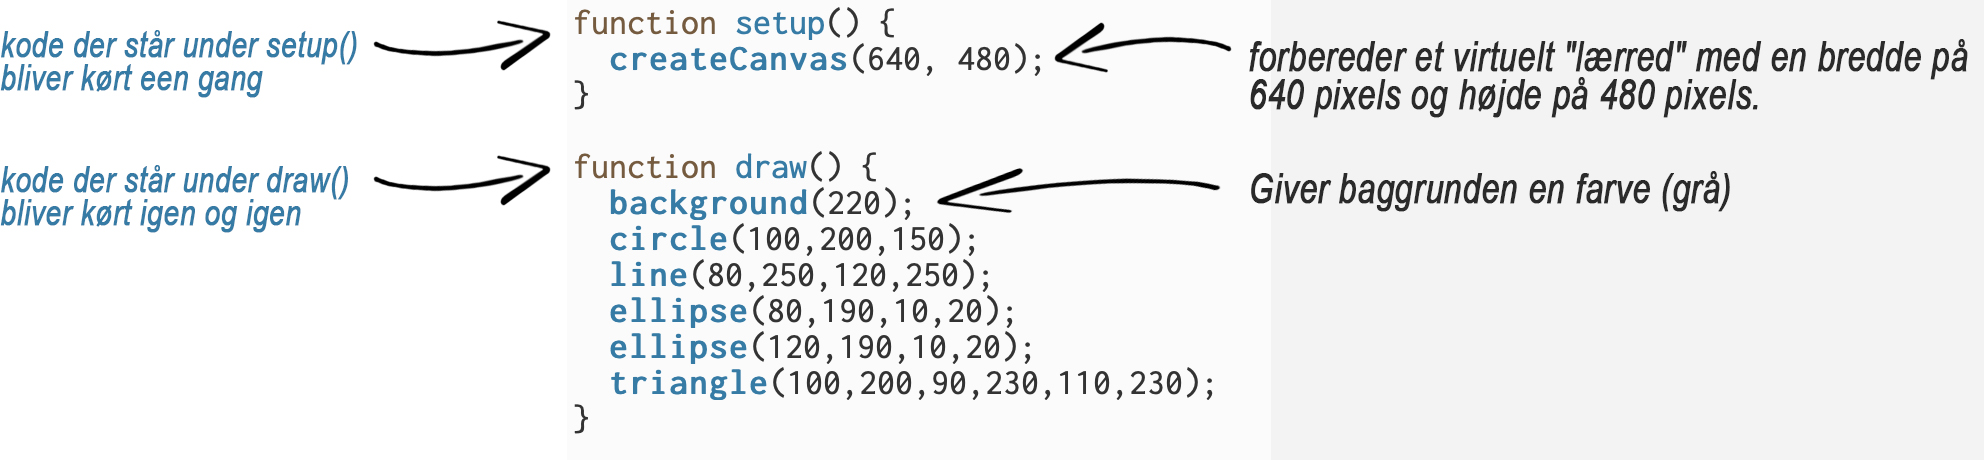
\includegraphics[width=0.90\textwidth]{nyebilleder/first.jpg} \\

Klik på 
\includegraphics[height=5mm]{ikoner/run.png}, og se hvad der sker. 
\vspace{3mm}

Gem projektet og kald det "tegning".\\

Tilføj nu følgende til draw-funktionen, nedenunder de linjer du allerede har skrevet, men før den sidste krøllede parentes \}:

\vspace{3mm}
\quad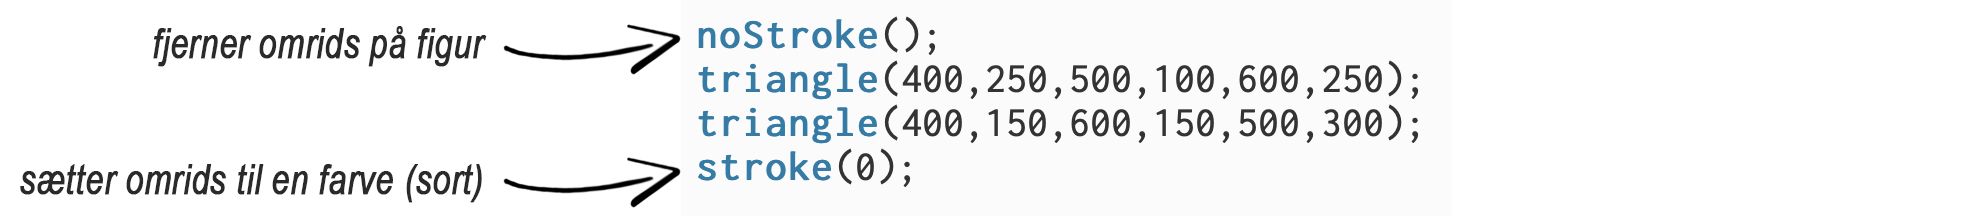
\includegraphics[width=0.85\textwidth]{nyebilleder/kodeeks.jpg} \\

Klik på 
\includegraphics[height=5mm]{ikoner/run.png}, og se hvad der sker. \\

Tilføj nedenstående til draw. Klik på 
\includegraphics[height=5mm]{ikoner/run.png} cirka halvejs og igen når det hele er skrevet ind:

\vspace{3mm}
\quad\quad\quad\quad\quad\quad\quad\quad\quad\quad\quad\quad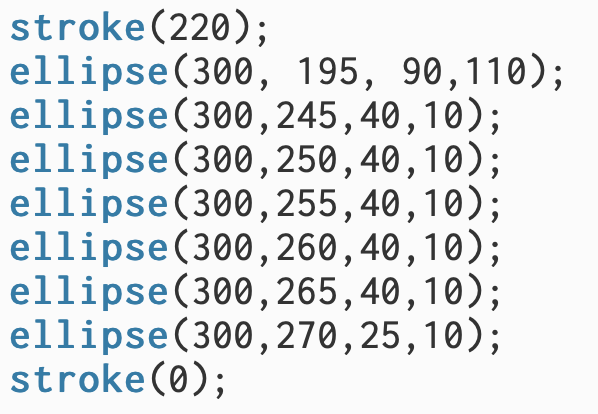
\includegraphics[width=0.27\textwidth]{nyebilleder/bulb.png} \\

\tcbsubtitle{Opgave}
\vspace{3mm}
Tegn 2-3 simple figurer - find gerne på dine egne!

\vspace{3mm}
\quad\quad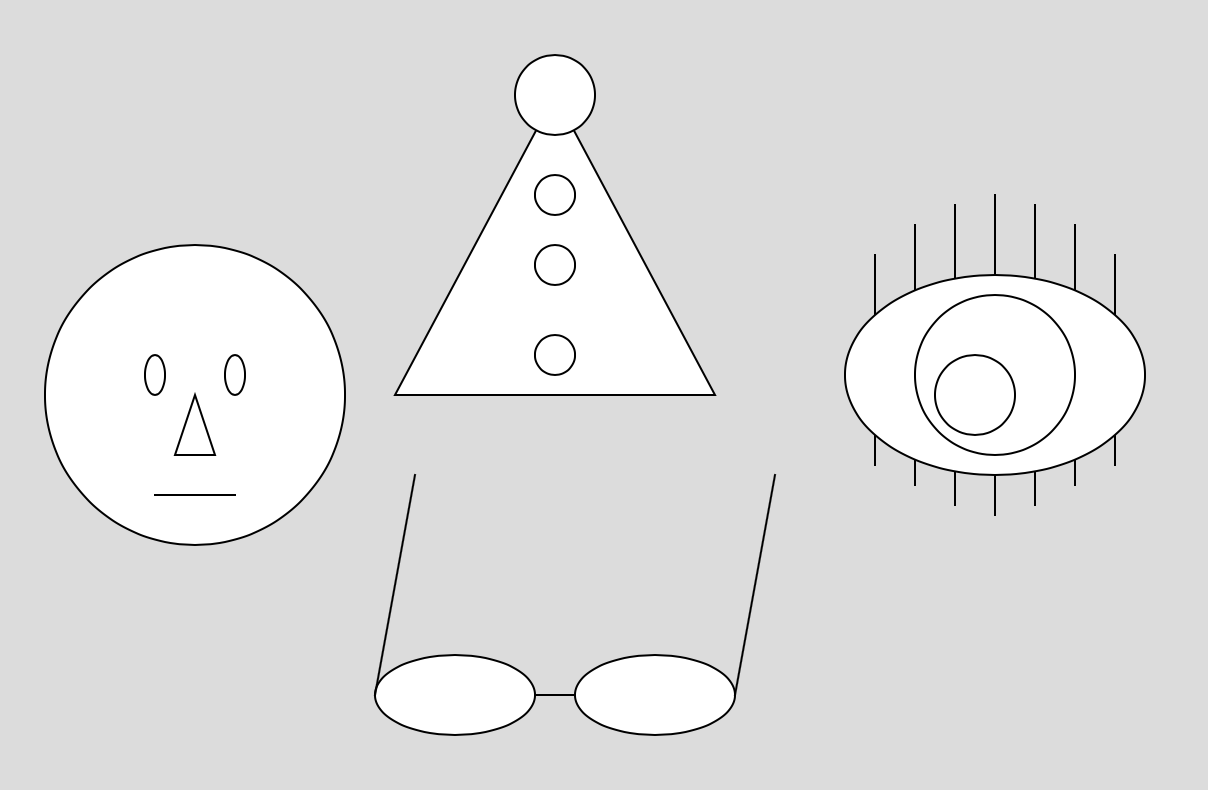
\includegraphics[width=0.35\textwidth]{nyebilleder/figurer.png} 

\end{exercisebox}

\newpage

\begin{exercisebox}[adjusted title=Farver]
\textit{Kodeeksemplet er med en enkelt cirkel, men du skal bare lade de figurer du har tegnet stå.}\\
Skriv følgende ind i din kode: 

\vspace{3mm}
\quad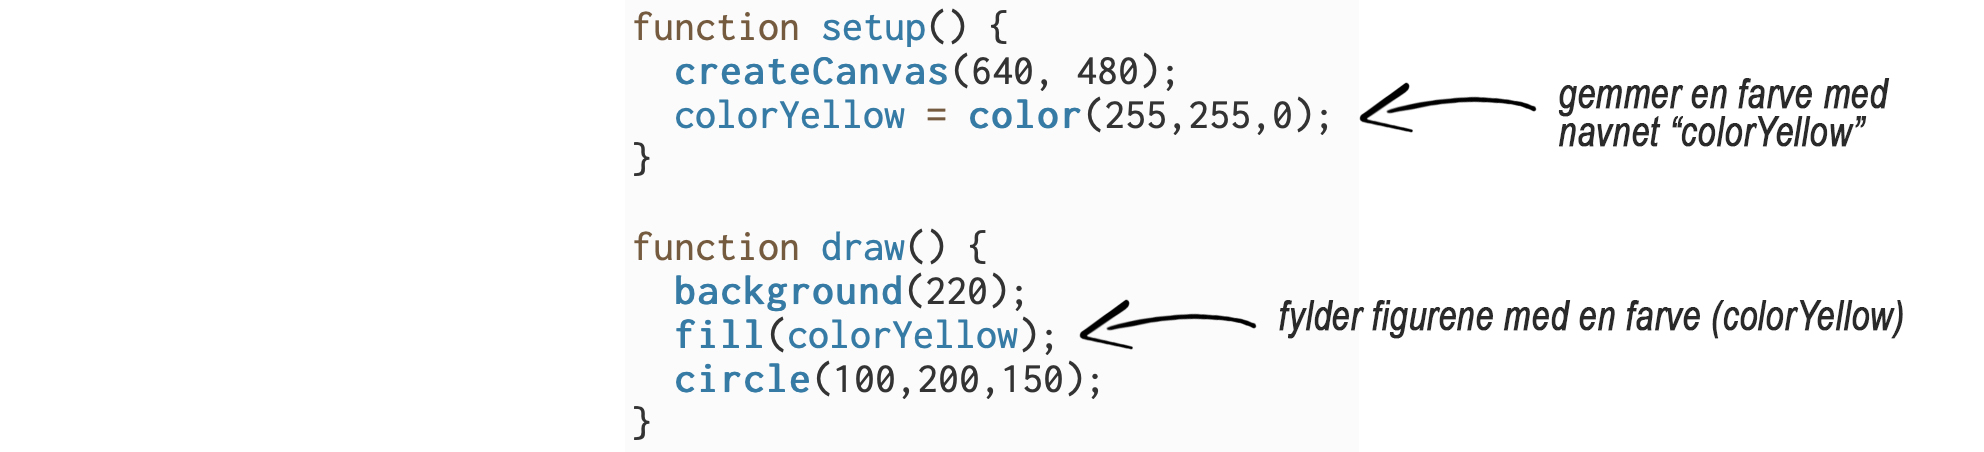
\includegraphics[width=0.85\textwidth]{nyebilleder/kodeeksfarver.jpg} \\



For at angive en farve skal farvens RGB-værdier bestemmes. RGB står for red-green-blue. Man skriver \textbf{color(}red , green ,blue\textbf{)} hvor red, green og blue er et tal mellem 0 og 255. \\
%Dette giver mulighed for 256 x 256 x 256 = 16.777.216 forskellige farver. \\
%Skal man bruge en gråtone, behøver man kun at angive et enkelt tal mellem 0 og 255.\\

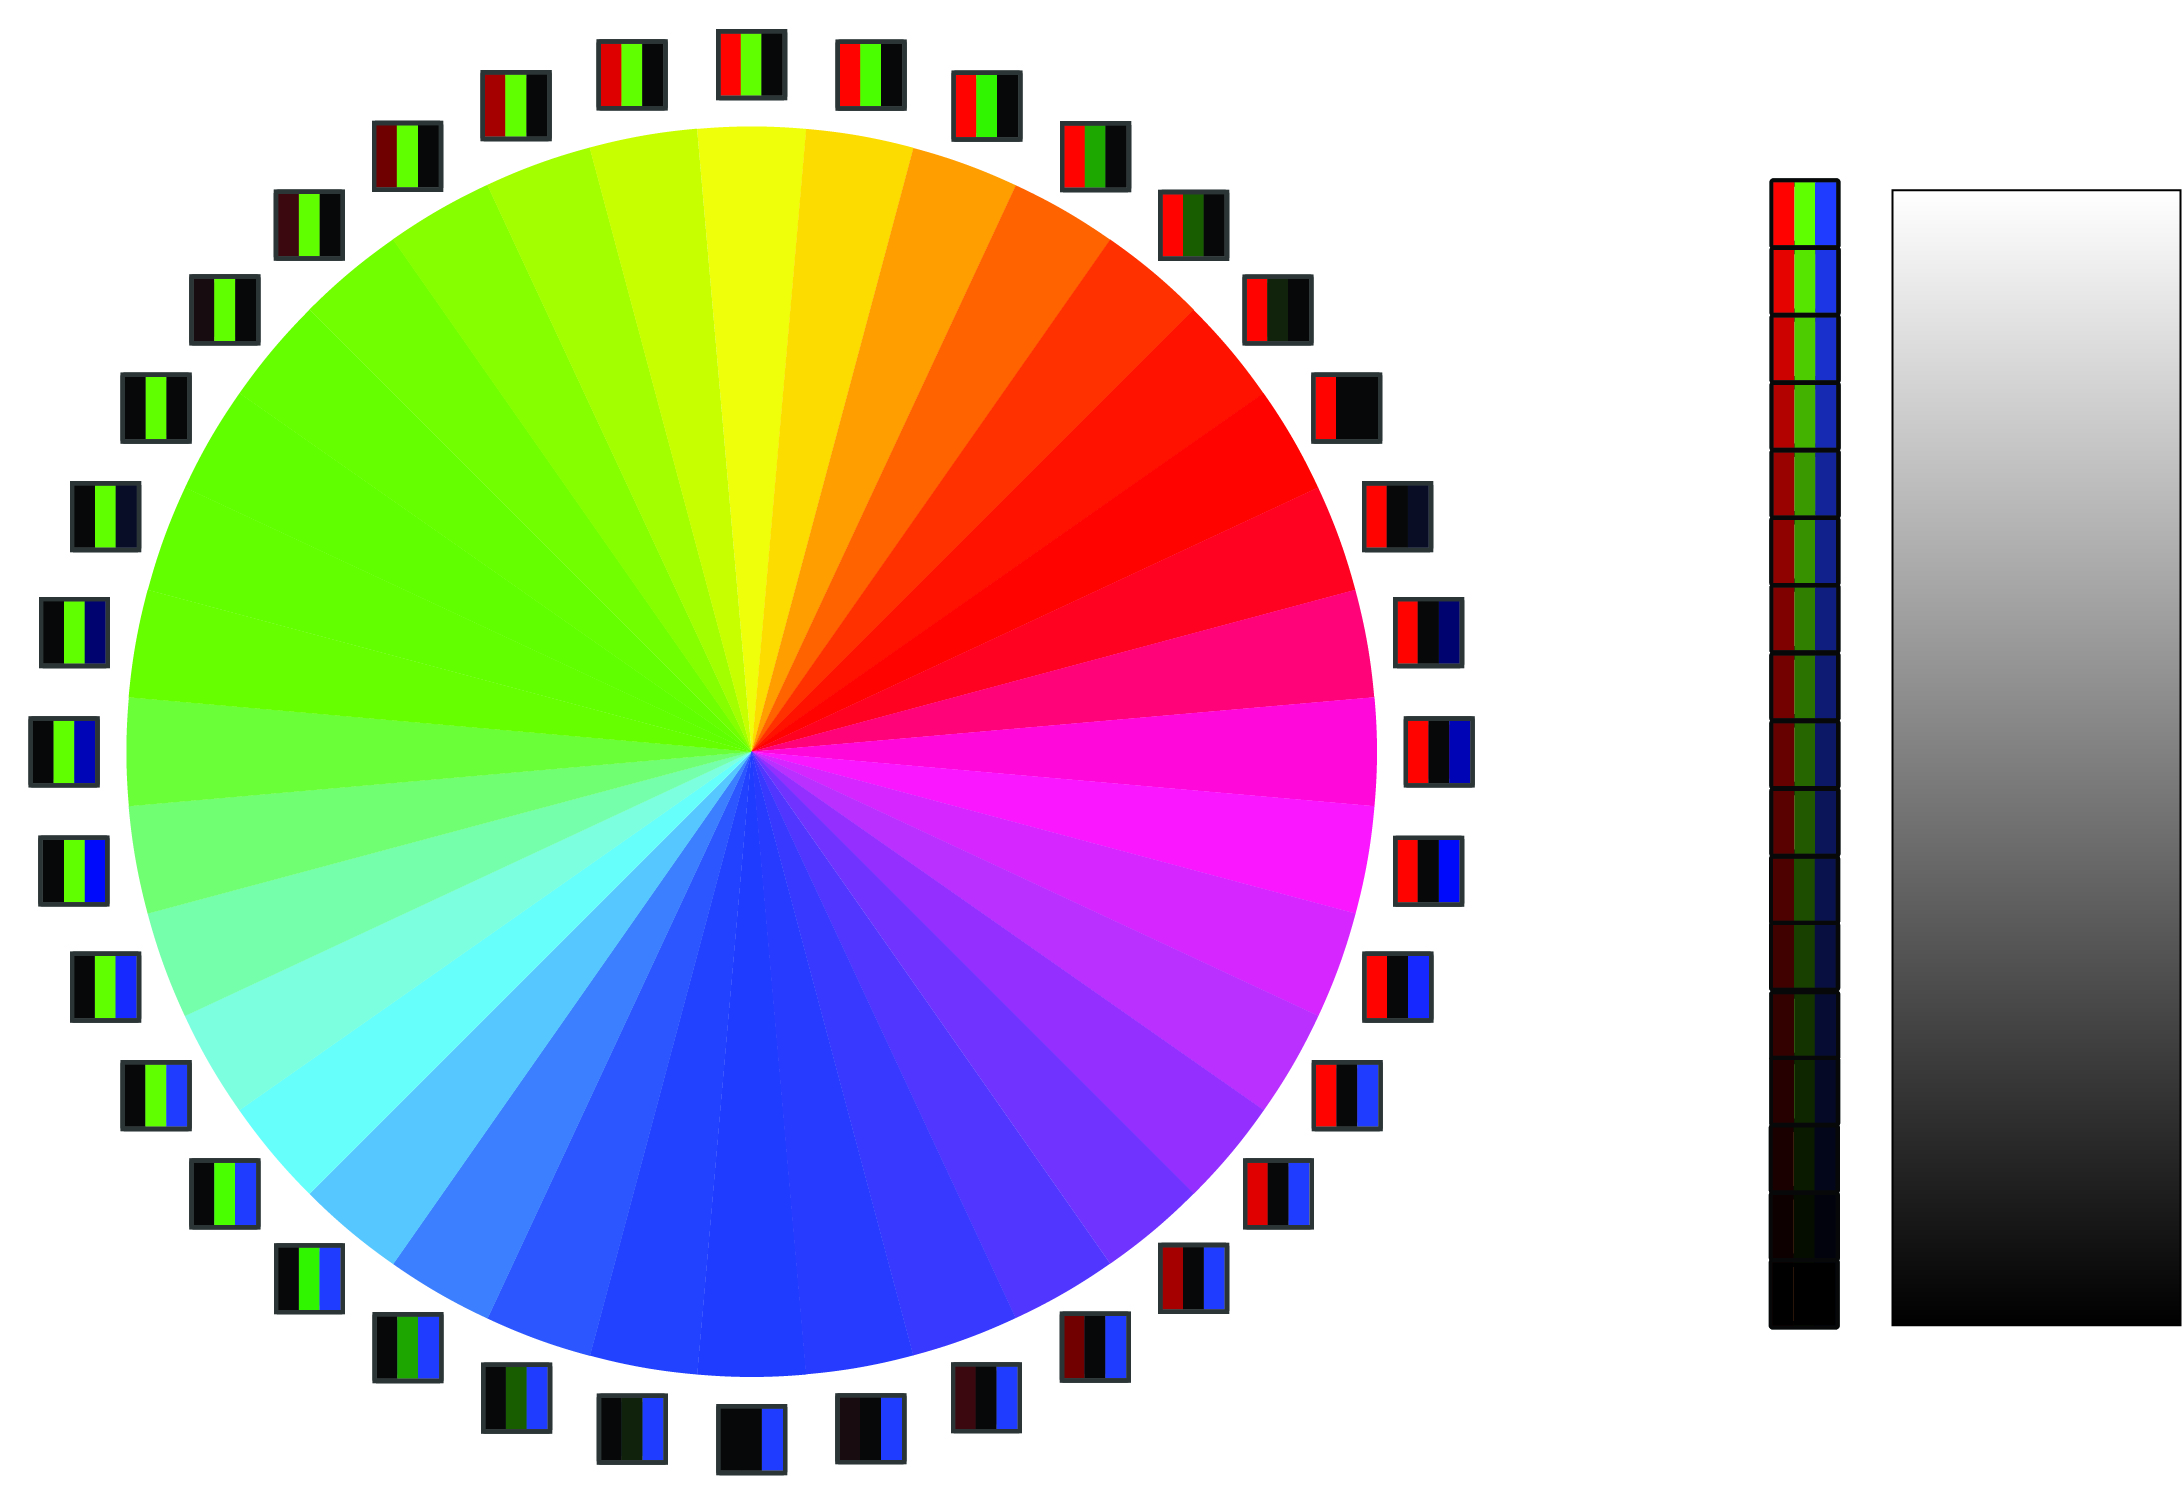
\includegraphics[width=0.4\textwidth]{billeder/rgbcolor.jpg} \\

Med \textbf{fill()} styrer hvilken farve du fylder dine figurer ud med. Du kan lave farver du kan genbruge i \textbf{setup()}, eller du kan skrive (r,g,b)-værdierne direkte som talværdier. \\

Du kan også skrive et enkelt tal for gråskala.\\

\quad\quad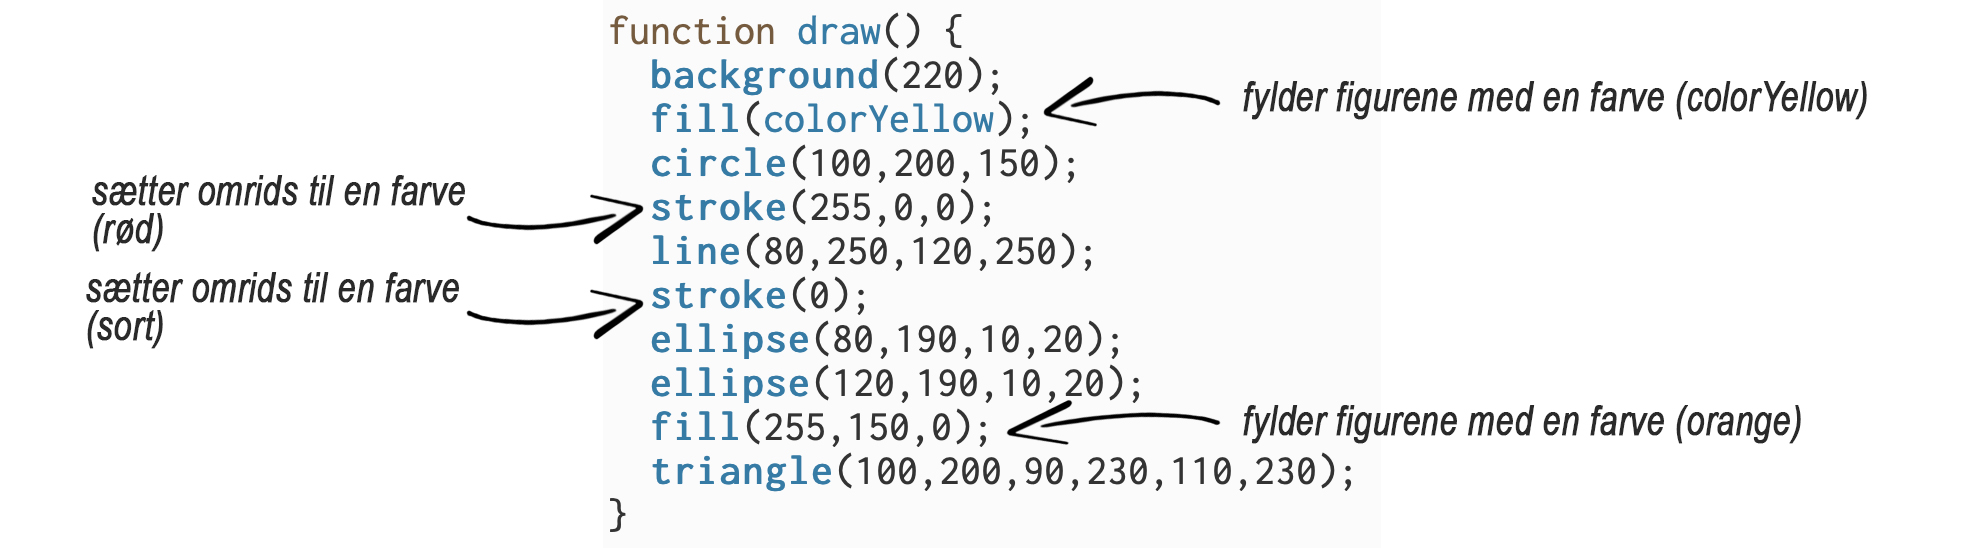
\includegraphics[width=0.85\textwidth]{nyebilleder/mereefarveeks.jpg} 

\vspace{3mm}
\noindent
\tcbsubtitle{Opgave}
\vspace{3mm}

Giv din tegning noget farve.\\

\quad\quad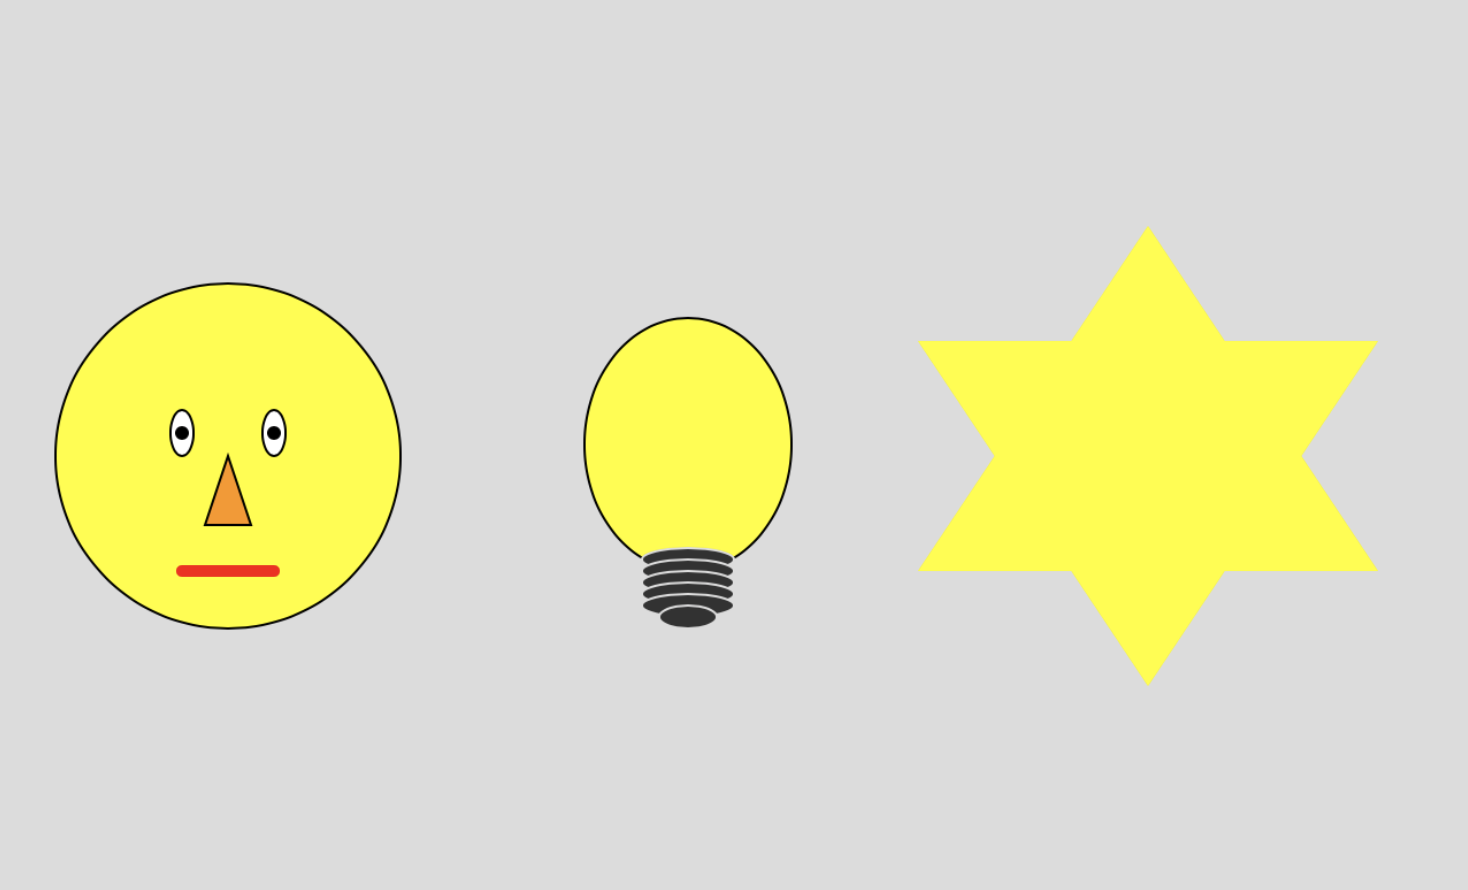
\includegraphics[width=0.35\textwidth]{nyebilleder/Screenshot 2021-04-15 at 11.40.20.png} 

\vspace{3mm}
\textit{På \url{https://p5js.org/reference/} kan du finde en oversigt over de vigtigste funktioner i p5js og en forklaring med eksempler på hvordan de bruges. }

\end{exercisebox}

\newpage
\stepcounter{handout}


\renewcommand{\Title}{\Ark Tilføj elementer}%


\begin{exercisebox}[adjusted title=Funktioner]

Åben p5js i et nyt faneblad og start en ny sketch.\\

Gem den nye sketch og kald den "funktioner".\\

Skriv følgende i din nye sketch:\\

\quad\quad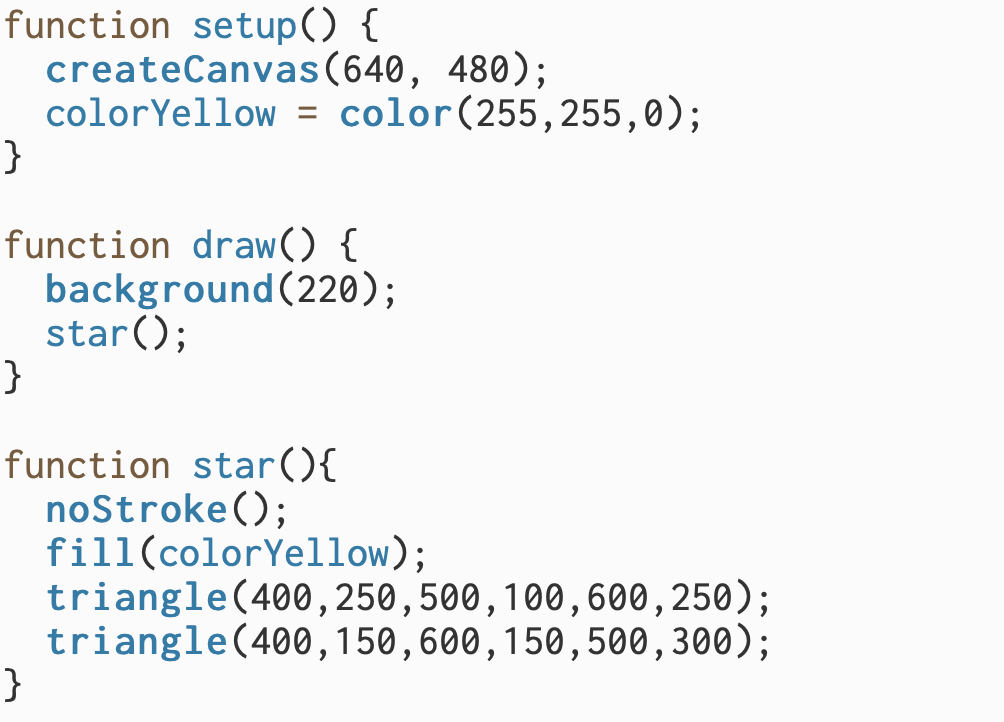
\includegraphics[width=0.45\textwidth]{nyebilleder/starfunktion.png} \\

For at kunne bevare overblikket i  \textbf{draw()}, samles noget af koden i en funktion.\\

En funktion laves ved at man skriver:\\ 

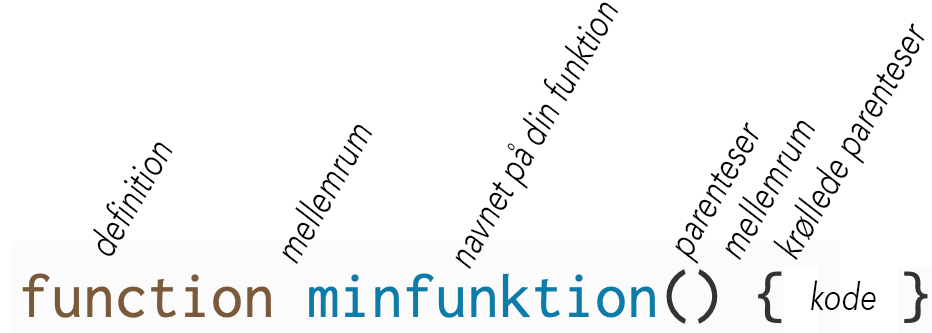
\includegraphics[width=0.8\textwidth]{nyebilleder/kodefunktion.jpg} \\

Imellem de to krøllede parenteser \{\} skrives al den kode der skal køres når man kalder funktionen. \\


Nu kan man nemt og overskueligt få tegnet sin tegning ved at skrive funktionens navn, efterfulgt af (); under funktionen \textbf{draw()} \\


\vspace{3mm}

\noindent
\tcbsubtitle{Opgave}

\vspace{3mm}
Skriv en funktion til hver af dine tegninger og få dem tegnet kun ved at skrive funktionernes navne under \textbf{draw()}  \\

\quad\quad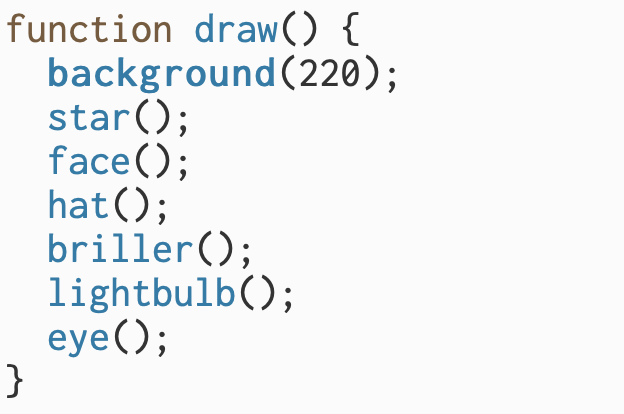
\includegraphics[width=0.3\textwidth]{nyebilleder/liste.png}

\end{exercisebox}



\newpage

\begin{exercisebox}[adjusted title=Billeder]
Download dette billede af fyrværkeri - det ligger på wikicommons, som er et godt sted at lede efter billeder hvis man ikke vil overtræde nogens copyright:

\vspace{3mm}
\quad \includegraphics[width=0.6\textwidth]{nyebilleder/fyrri2.png}\\ 
\url{https://upload.wikimedia.org/wikipedia/commons/0/04/Firework_transparent.png} \\

Åbn sketchfiles, vælg "Upload file" og find fyrværkeribilledet der hvor du gemte det.\\

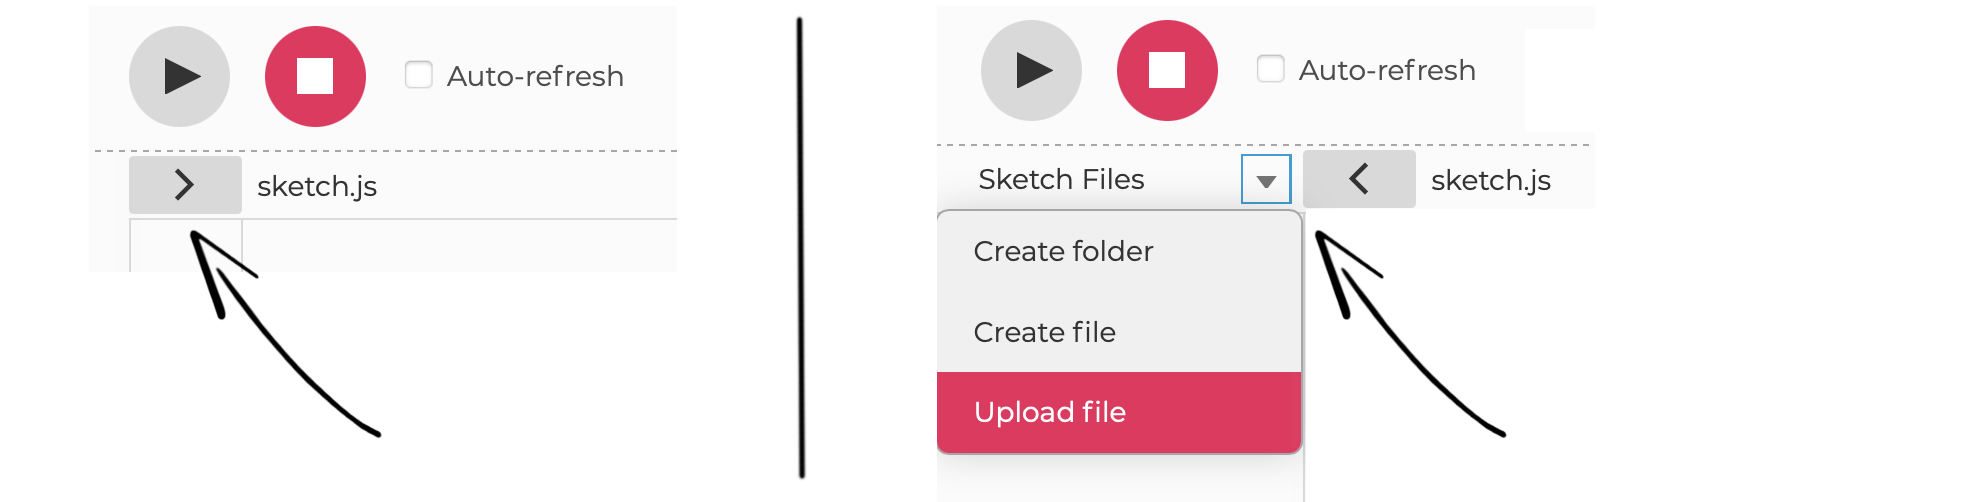
\includegraphics[width=0.8\textwidth]{nyebilleder/topile.jpg} \\

Skriv følgende i din kode:\\

\quad\quad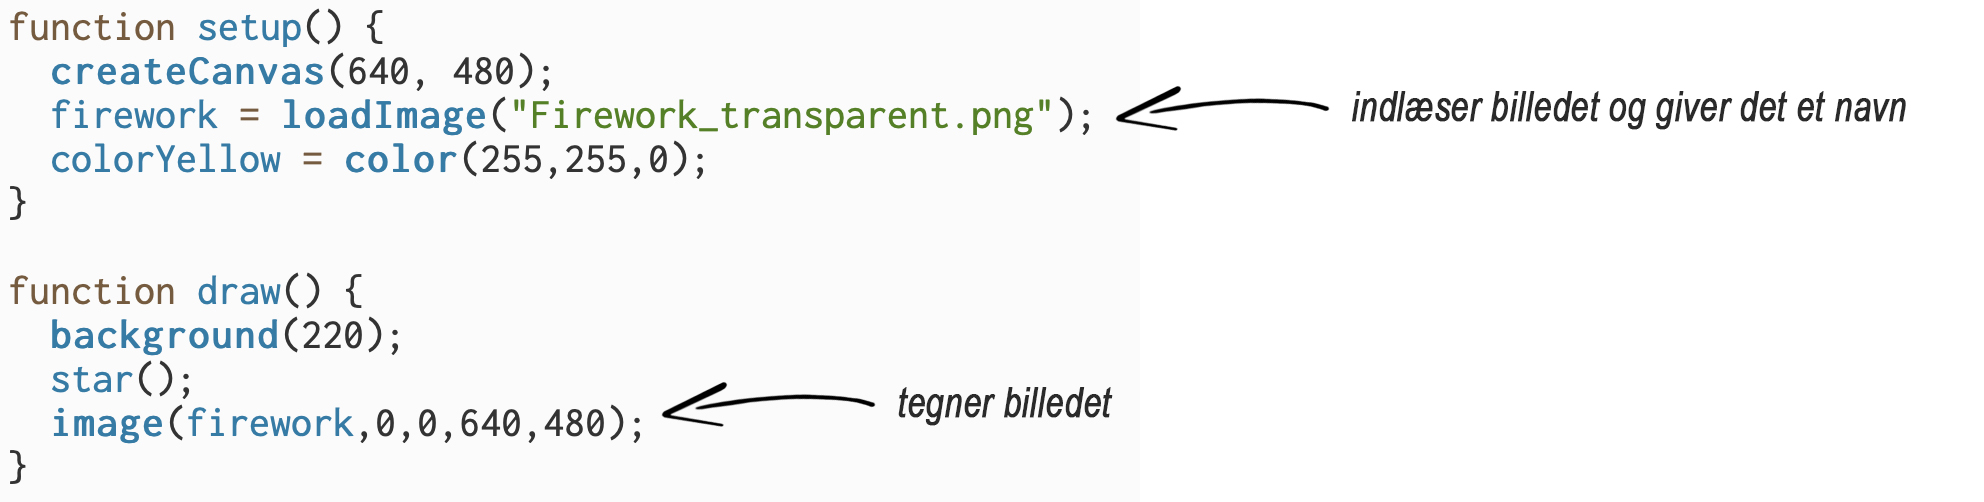
\includegraphics[width=0.8\textwidth]{nyebilleder/billedekode.jpg} \\

Når du tegner billedet under \textbf{draw()} bruger du en funktion der hedder \textbf{image()}. \\

I parenteserne efter \textbf{image} står først navnet på dit billede, de to tal der står efter navnet, er x og y koordinatet til øverste venstre hjørne. Du behøver ikke at give flere tal med, men hvis dit billede er for stort, kan du give to tal mere med, nemlig den ønskede bredde og højde. 
\vspace{3mm}

\tcbsubtitle{Opgave}
\vspace{3mm}
Find selv et billede og sæt det ind i din kode.

\end{exercisebox}


\newpage

\begin{exercisebox}[adjusted title=Video]
\textit{Særligt til Windowsbrugere: Windows tillader kun at kameraet bliver brugt et sted af gangen, det kan derfor være du bliver nødt til at slå video fra i Zoom for at få koden til at virke i p5js}\\

Vi bruger den indbyggede funktion \textbf{createCapture(VIDEO)} til at starte vores webcam. Skriv følgende kode ind: \\

\quad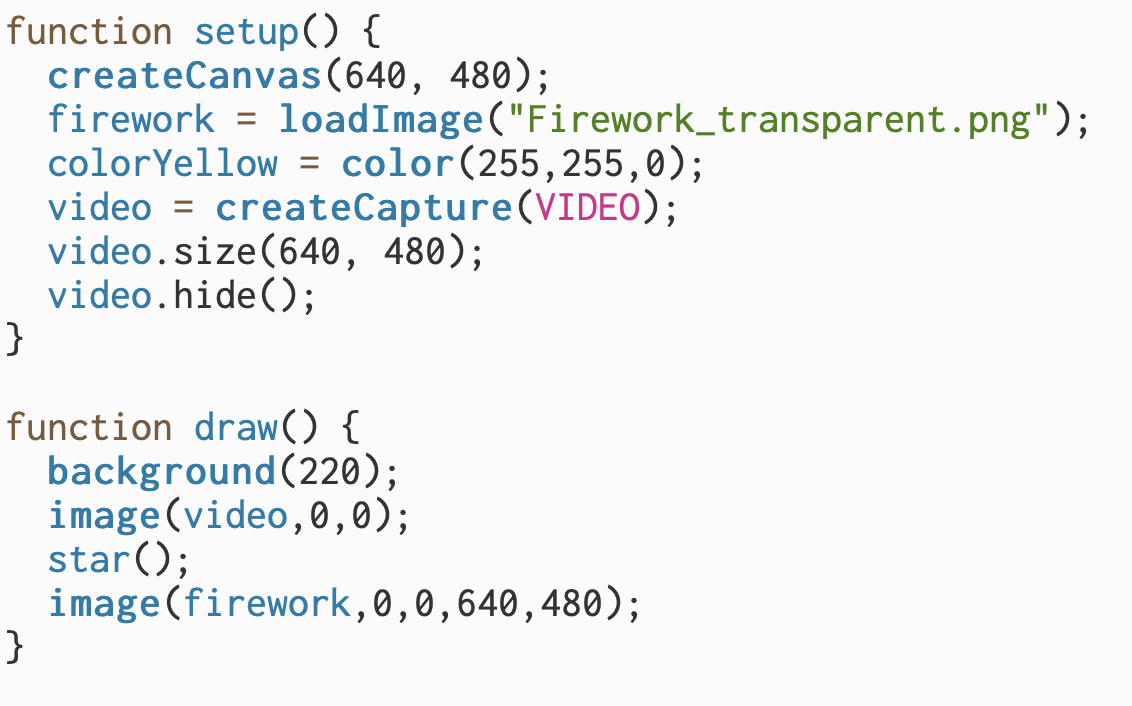
\includegraphics[width=0.5\textwidth]{nyebilleder/vidoeplus.png} \\

Størrelsen på videooptagelsen sættes til samme størrelse som vores lærred. Sidste linje i \textbf{setup()} skjuler et preview af videoen, men den optager stadig.\\

For at vise videoen på lærredet, skal den tegnes i \textbf{draw()}. Det foregår på samme måde som når man tegner et billede. De to tal efter navnet er koordinaterne til øverste venstre hjørne. Vi har allerede angivet størrelsen, så det behøver vi ikke at gøre igen.
\vspace{3mm}
\tcbsubtitle{Opgave}
\vspace{3mm}
Sæt de forskellige elementer vi har arbejdet med indtil nu sammen, så der både bliver tegnet video, billeder og de tegninger du har lavet med kode. Fordel tegninger og billeder lidt dekorativt omkring dit videobillede. 

\begin{center}
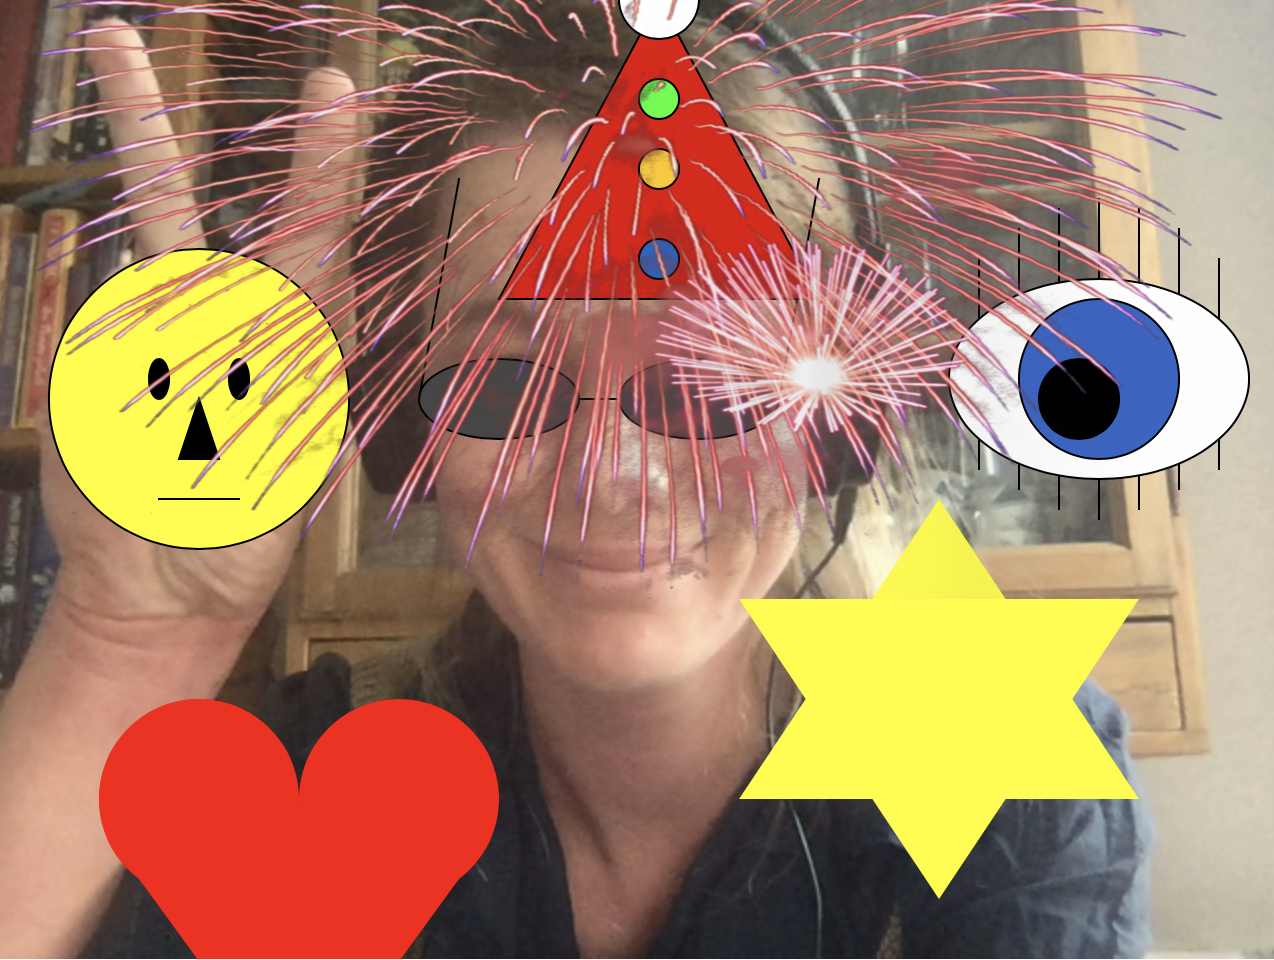
\includegraphics[width=0.6\textwidth]{nyebilleder/coolpi.png}
\end{center}
\end{exercisebox}

\newpage

\stepcounter{handout}

\renewcommand{\Title}{\Ark Virtuelt kamera}%

\begin{exercisebox}[adjusted title= Start virtuelt kamera]
\textbf{p5js:}\\
Start med at gemme din sketch, hvis du ikke allerede har gjort det. Dernæst under \textbf{File} vælges \textbf{Share} og \textbf{Fullscreen}. Åbn linket i et nyt vindue.  \\

\textbf{OBS:}\\
Download OBS - Open Broadcaster Software her: \url{https://obsproject.com}\\ 
Installer og åbn.\\

Hvis den sige noget om automatisk guide til opsætning, så tryk annuller.\\ 

Tryk på \textbf{+} for at tilføje en ny \textbf{source}/\textbf{kilde} og vælg \textbf{Window capture}/\textbf{vinduesoptagelse}. \\

Vælg det vindue der kører din kode.\\

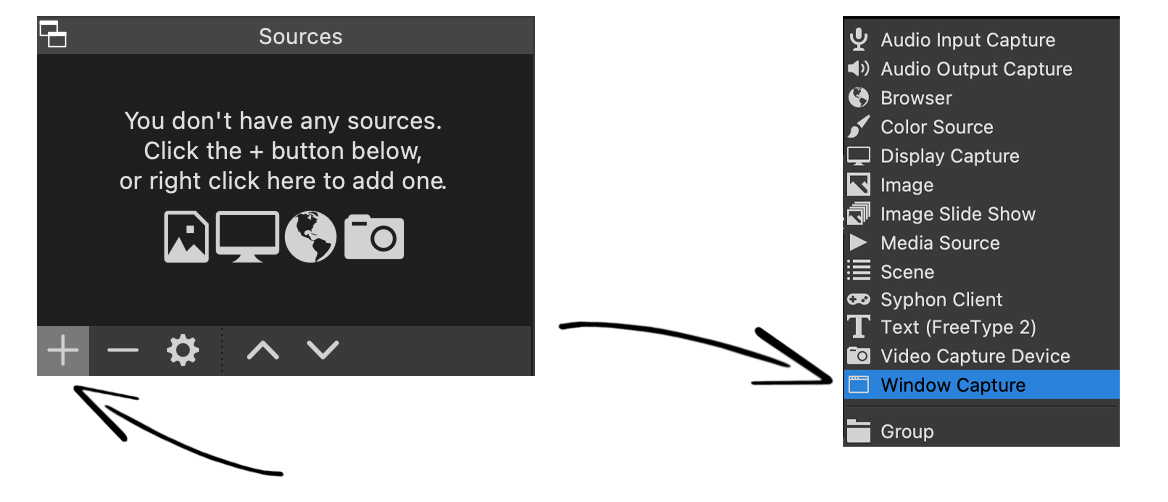
\includegraphics[width=0.7\textwidth]{nyebilleder/sourses.jpg}\\

Beskær billedet i OBS ved at holde \textbf{Option-tasten} inde på Mac eller \textbf{Alt} inde på Windows og træk i de røde punkter i rammen. Klip til så det kun er videobilledet der ses. Du skalerer ved at trække i de røde punkter uden at Option/Alt er holdt nede. \\

Nu mangler du kun at starte virtuelt kamera i OBS (under \textbf{Controls}/\textbf{Styring}) \\

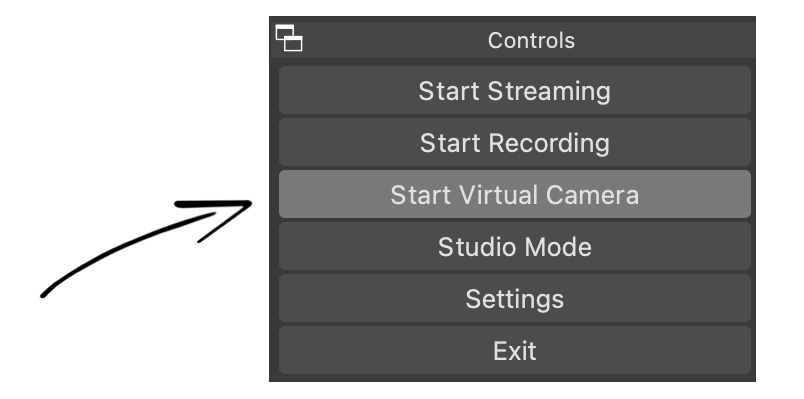
\includegraphics[width=0.45\textwidth]{nyebilleder/virtu.jpg}\\
\textbf{Zoom:}\\
Dit virtuelle kamera skulle gerne dukke op som et kamera der kan vælges i Zoom. Sandsynligvis skal Zoom genstartes.\\

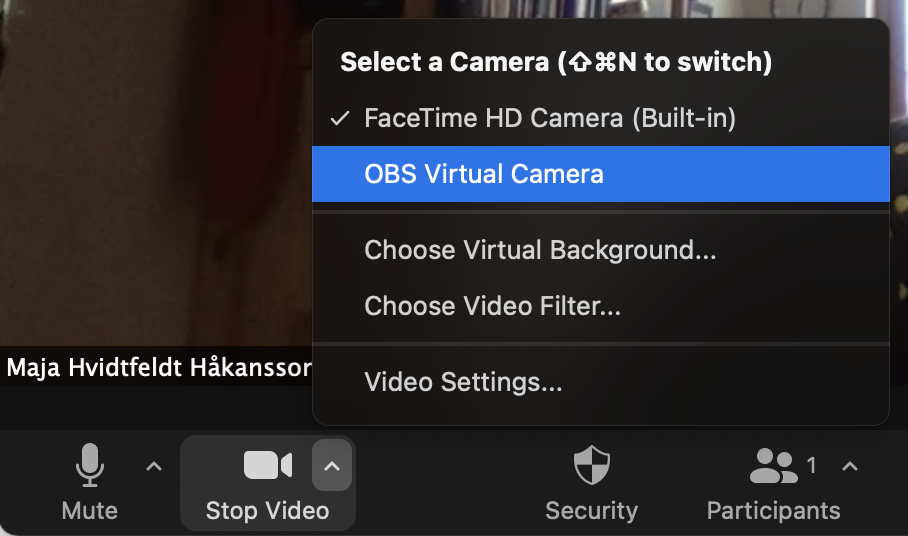
\includegraphics[width=0.45\textwidth]{nyebilleder/virtueltzoom.png}\\
\end{exercisebox}

\newpage

\stepcounter{handout}
\renewcommand{\Title}{\Ark Machine Learning}%
\begin{exercisebox}[adjusted title= Teachable Machine] 

\textit{Der kan være lidt forskel på hvordan Teachable Machine virker i de forskellige browsere. Hvis det ikke fungere optimalt, så prøv at bruge en anden browser.}\\

Gå til \url{https://teachablemachine.withgoogle.com} \\


Tryk på den store blå knap for at komme i gang: \raisebox{-2mm}{
\includegraphics[width=0.15\textwidth]{ikoner/teachablemachinestart.png}}\\

Klik på \textbf{Image Project} for at lave en model der er baseret på billeder:

\quad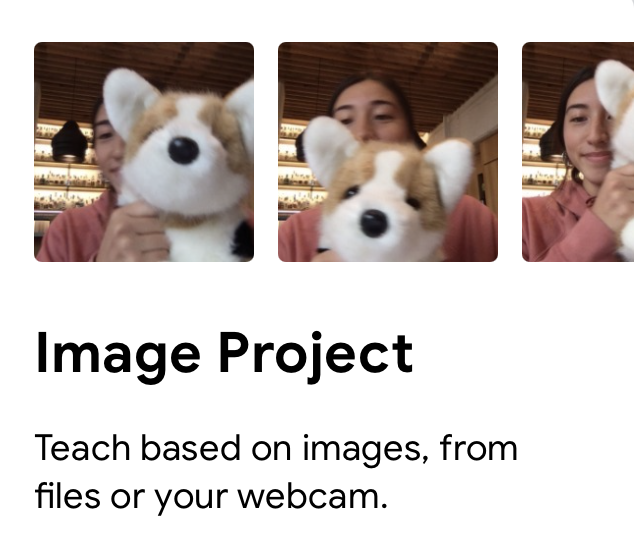
\includegraphics[width=0.18\textwidth]{billeder/imageproject.png}

Start med at omdøbe \textbf{Class 1} til \textbf{Normal} og klik derefter på: \raisebox{-2mm}{
\includegraphics[width=0.08\textwidth]{ikoner/webcam.png}}

Hold knappen \raisebox{-1mm}{
\includegraphics[width=0.17\textwidth]{ikoner/record.png}} nede mens du tager en masse billeder hvor du ser "normal" ud. Drej dig lidt, kig lidt til siden og læn dig frem, som du ville gøre når du normalt deltager i virtuel undervisning. \\

Omdøb nu \textbf{Class 2} til \textbf{handup} og tag en serie billeder hvor du har hånden oppe. Du skal tage omkring 200 billeder i hver klasse. \\

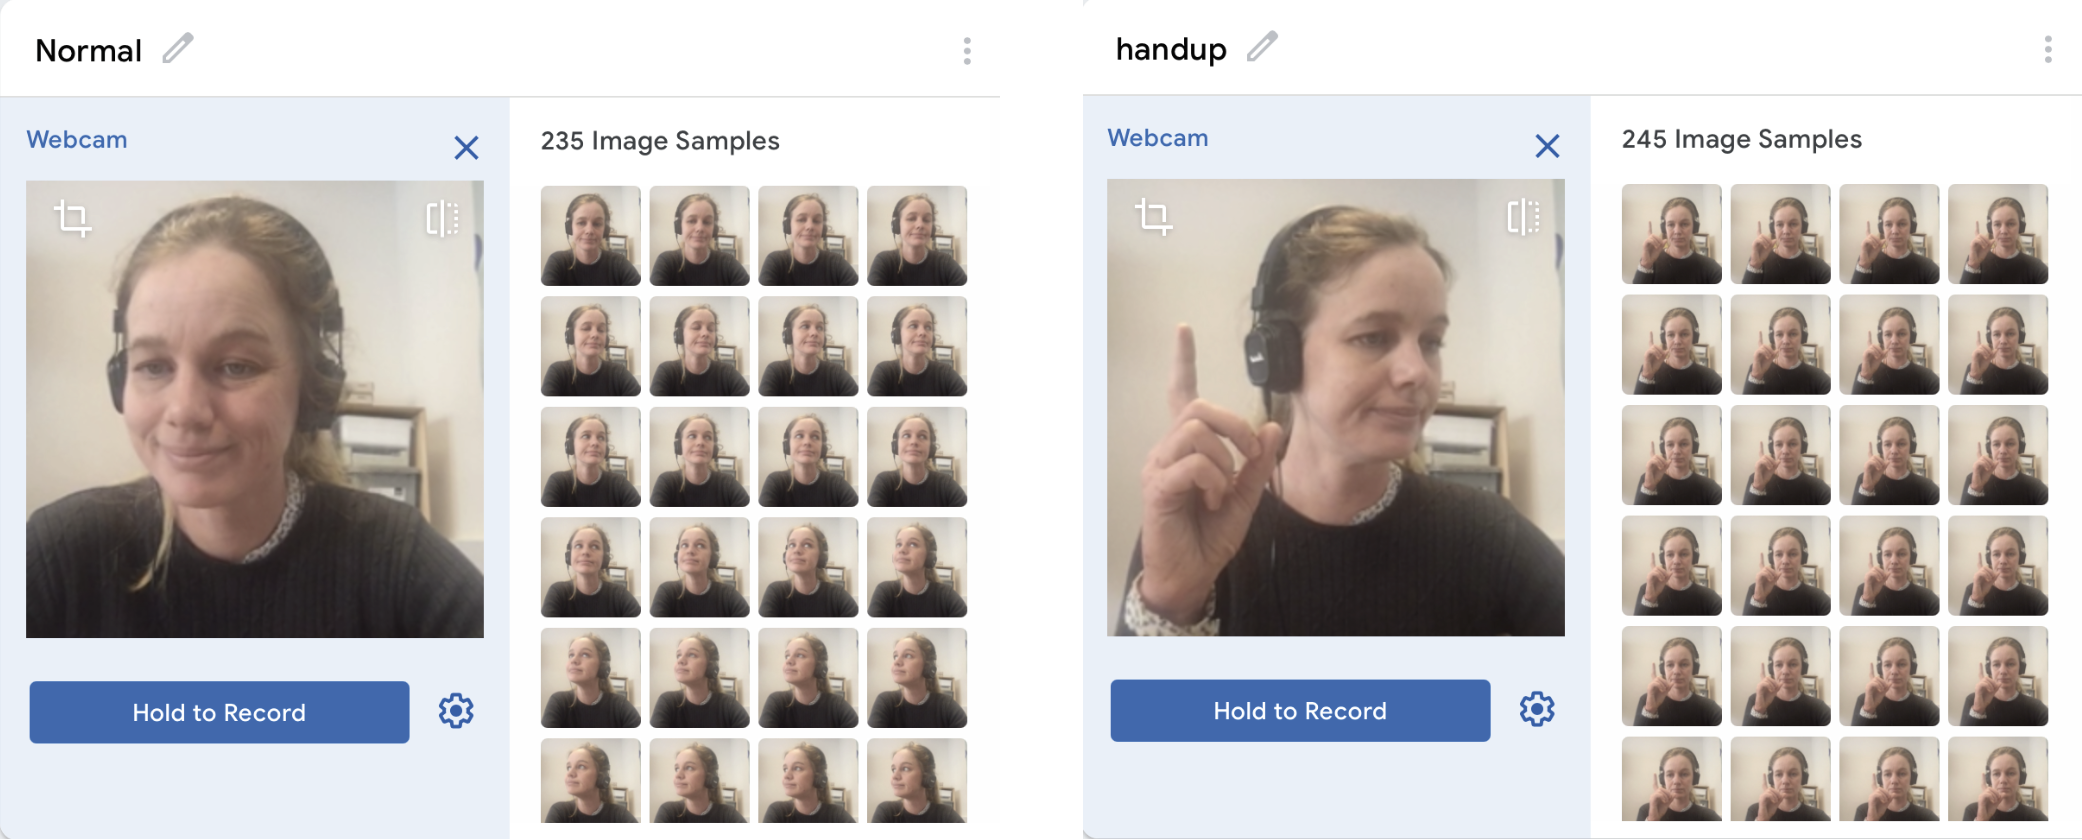
\includegraphics[width=1\textwidth]{billeder/training.png}\\

Derefter klikker du på \textbf{Train model} og venter tålmodigt på at den bliver færdig.

\begin{center}
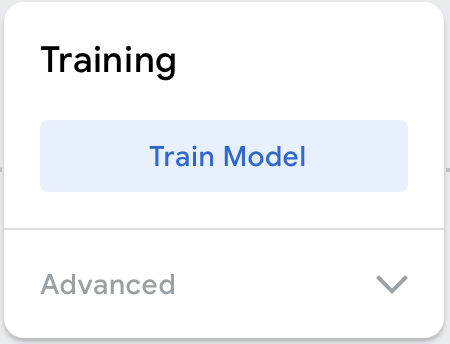
\includegraphics[width=0.2\textwidth]{billeder/trainmodel.png}
\end{center}

Når modellen er trænet, kan du se hvor godt det virker med de billeder du har givet. 


\includegraphics[width=0.30\textwidth]{ikoner/prcent.png}

Den skulle gerne kunne skelne med en 95-100\% sikkerhed - ellers må du tage nye billeder og sikre dig der er forskel på de billeder der ligger i de to klasser. 

\end{exercisebox}

\newpage
\begin{exercisebox}[adjusted title= Exporter model]



For at kunne bruge din model skal du klikke på \textbf{Export Model} 
\includegraphics[width=0.2\textwidth]{ikoner/export.png} og derefter på \textbf{Upload my model}\\ 
\includegraphics[width=1\textwidth]{ikoner/uploadmodle.png}\\

Du får nu et link til din model. Kopier linket. \\
\vspace{3mm}

\noindent
\tcbsubtitle{Tilhørende kode i p5.js}
\vspace{3mm}
I et nyt faneblad åbner du dette link: \\

\url{https://editor.p5js.org/MajaHvidtfeldt/sketches/QZGHqB-fW}\\

Sketchen indeholder den kode og de funktioner der skal til for at vores billedegenkendelse virker. \\

Sæt dit link fra Teachable Machine ind i koden\\


\includegraphics[width=0.5\textwidth]{nyebilleder/linktcopy.png}\\

\textit{Hvis du bruger Windows, skal du skal være opmærksom på at at du ikke kan have Teachable Machine kørende i baggrunden samtidig med at du bruger video i p5.js}\\

\tcbsubtitle{Opgave}
\vspace{3mm}
Du skal flytte alle de funktioner du har lavet over i den nye sketch. Husk også at flytte det du har skrevet under \textbf{setup}. Du skal også uploade eventuelle billedfiler igen. \\

Du skal \textit{ikke} flytte det du eventuelt har stående under \textbf{draw()}. \\


\includegraphics[width=0.5\textwidth]{nyebilleder/heartcopy.png}


\end{exercisebox}



\newpage
\begin{exercisebox}[adjusted title=Tjek betingelse med \textit{if-statement}]

Nå du kører din kode nu, vil classifieren automatisk løbende lægge navnet på det den genkender dit billede som, ind i \textbf{label}, så hvis vi tjekker hvad label er, kan vi kæde det sammen med bestemte handlinger. \\

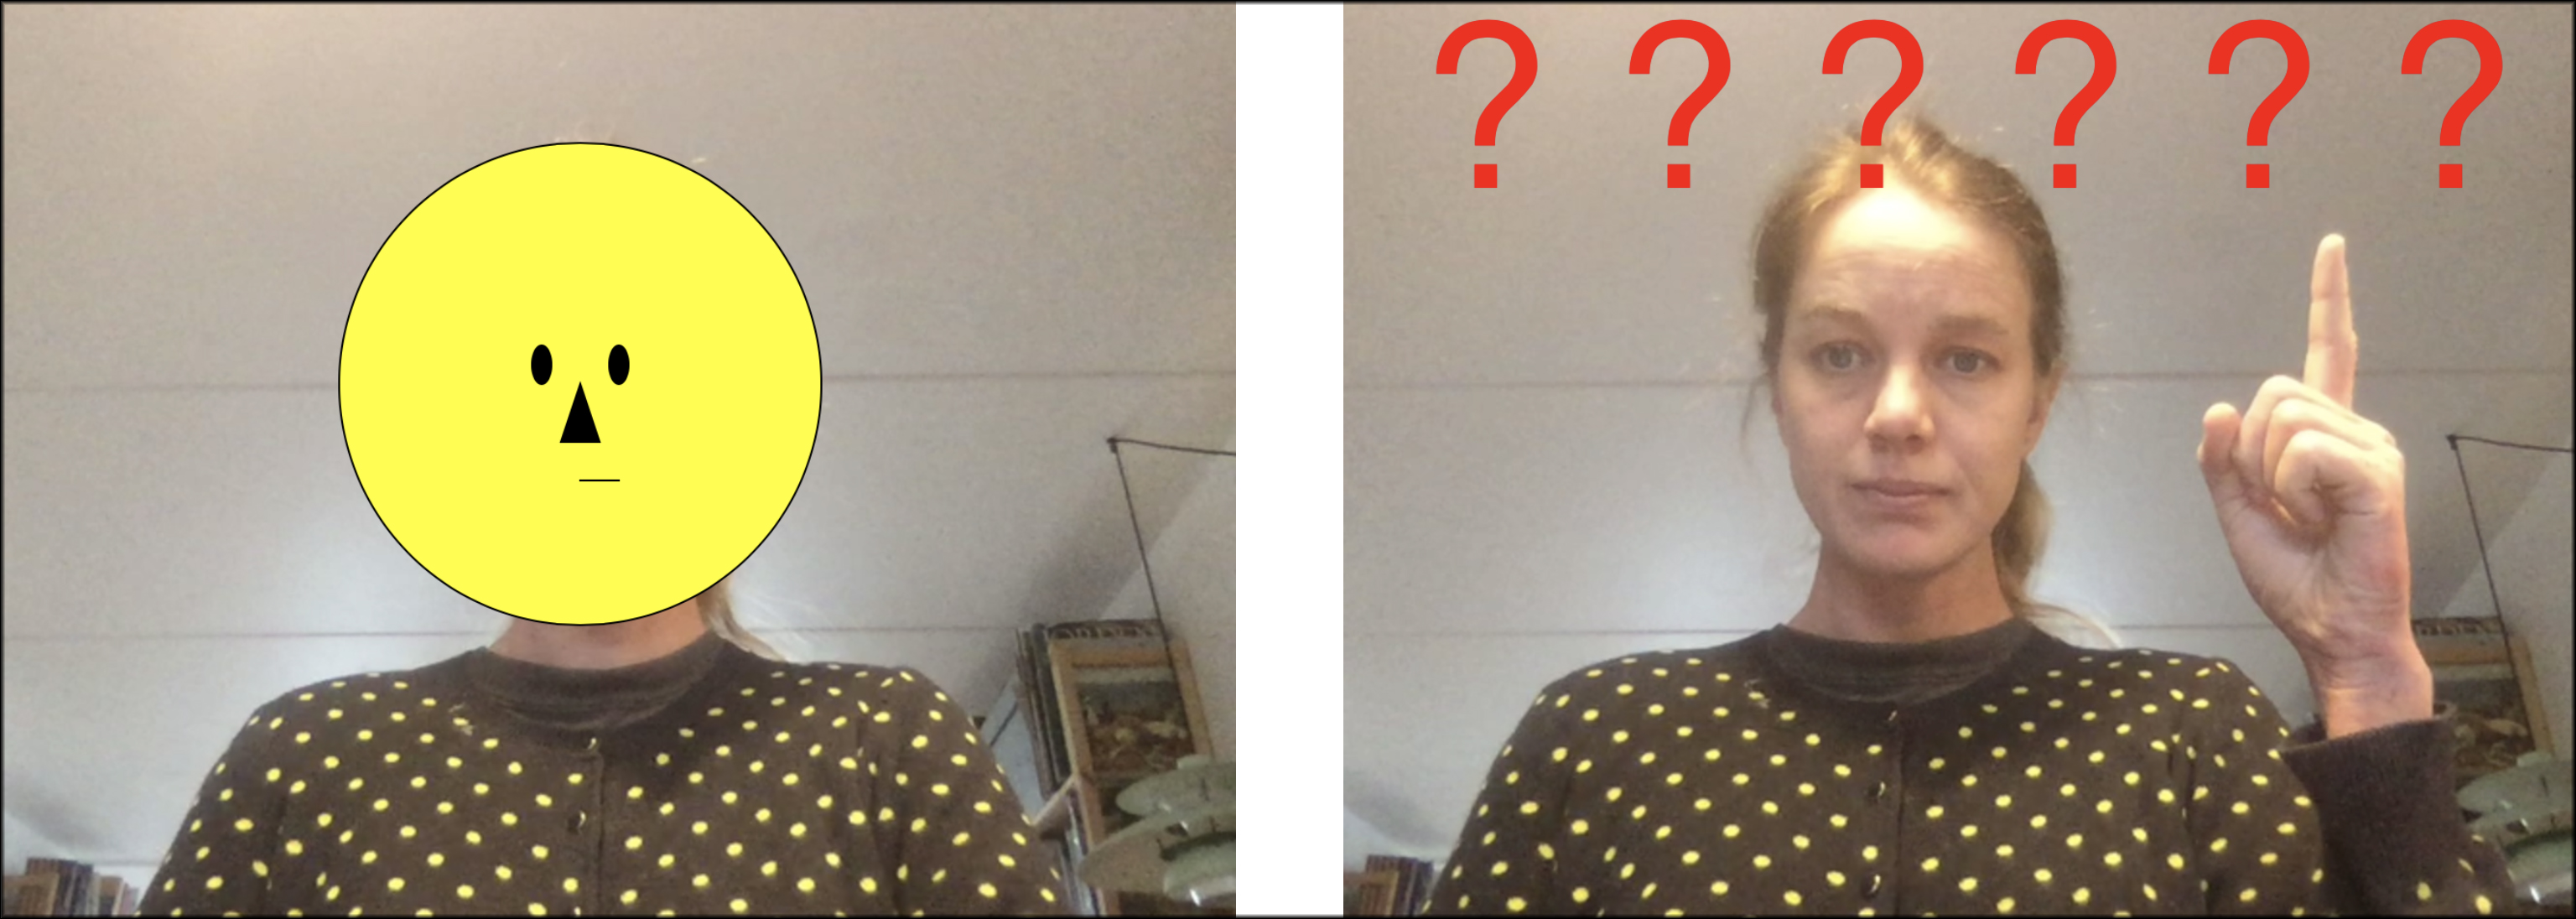
\includegraphics[width=0.7\textwidth]{nyebilleder/to.jpg} \\

Vi havde som udgangspunkt 2 klasser \textbf{Normal} og \textbf{handup}. Jeg kunne godt tænke mig at det ansigt jeg tidligere har tegnet bliver vist, når billedet klassificeres som "Normal", og at der kommer store røde spørgsmålstegn op, når jeg rækker fingeren i vejret. \\

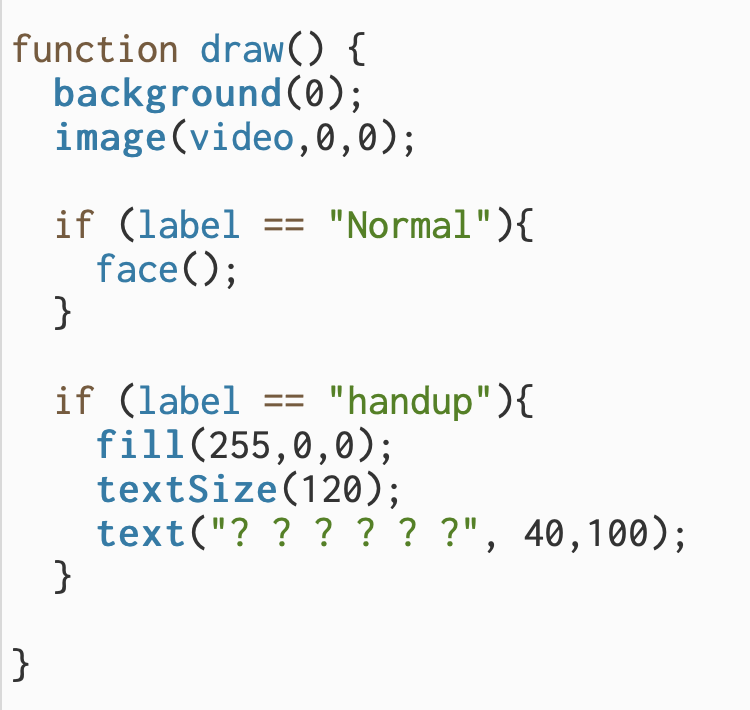
\includegraphics[width=0.4\textwidth]{nyebilleder/nukode.png} \\

Nu skal du bare, på samme måde som tidligere starte det virtuelle kamera i OBS - og dine videomøder vil aldrig blive det samme igen!! 

\tcbsubtitle{Opgave}
Du kan træne en ny model med flere klasser, eksportere den og erstatte \\ \textbf{imageModelURL}-linket i din kode med linket til den nye model.  \\
Du skal bare lave et \textbf{if-statement} til hver af dine klasser.\\

Måske er wauw-effekten størst hvis der ikke sker noget når \textbf{label == "Normal"}, men du bestemmer helt selv. Fra nu af og resten af workshoppen er der kun een opgave - at have det sjovt med billeder og kode!  \\

\hspace{4.5cm} 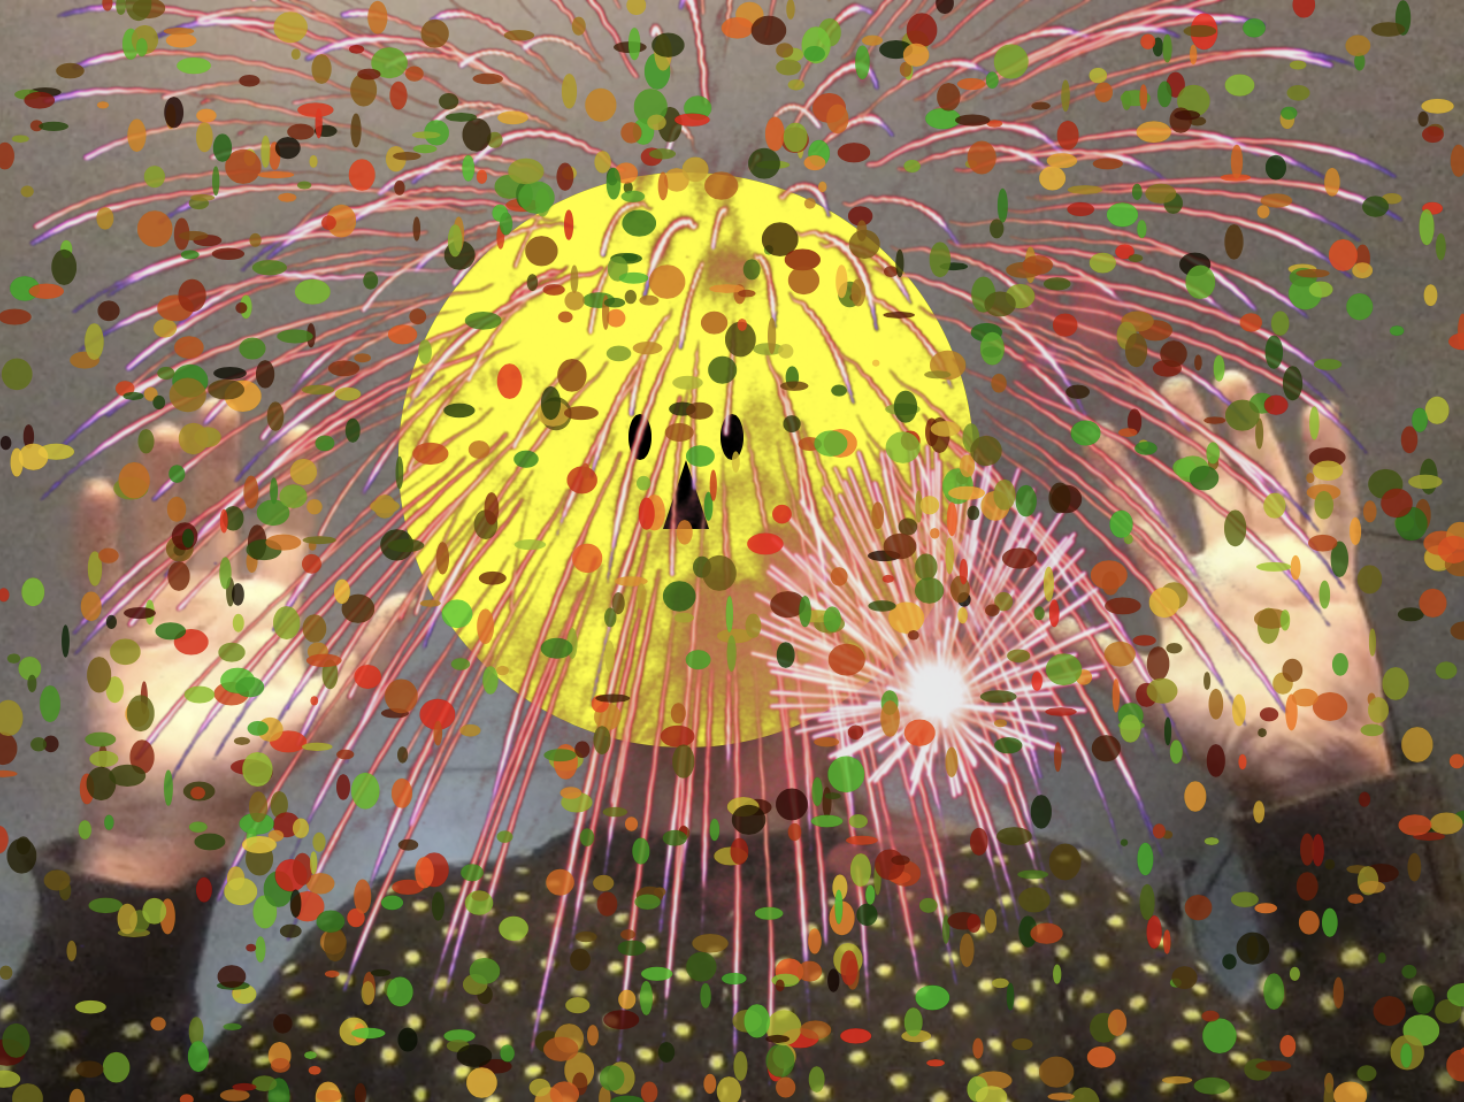
\includegraphics[width=0.35\textwidth]{nyebilleder/fest.png} \\

\end{exercisebox}

\newpage
\stepcounter{handout}
\renewcommand{\Title}{\Ark Appendix}%



\begin{exercisebox}[adjusted title= APPENDIX]
Her er samlet nogle af de ting vi overvejede at have med i workshoppen, men var nødt til at pille ud. Det er ikke gennemarbejdede ark, men vi tænkte at de er jer der er blevet nysgerrige på mere, måske kunne komme skridte videre ved hjælp af dem. 
\vspace{3mm}

\tcbsubtitle{Funktion med input}
Når man laver funktioner kan man give dem input. \\

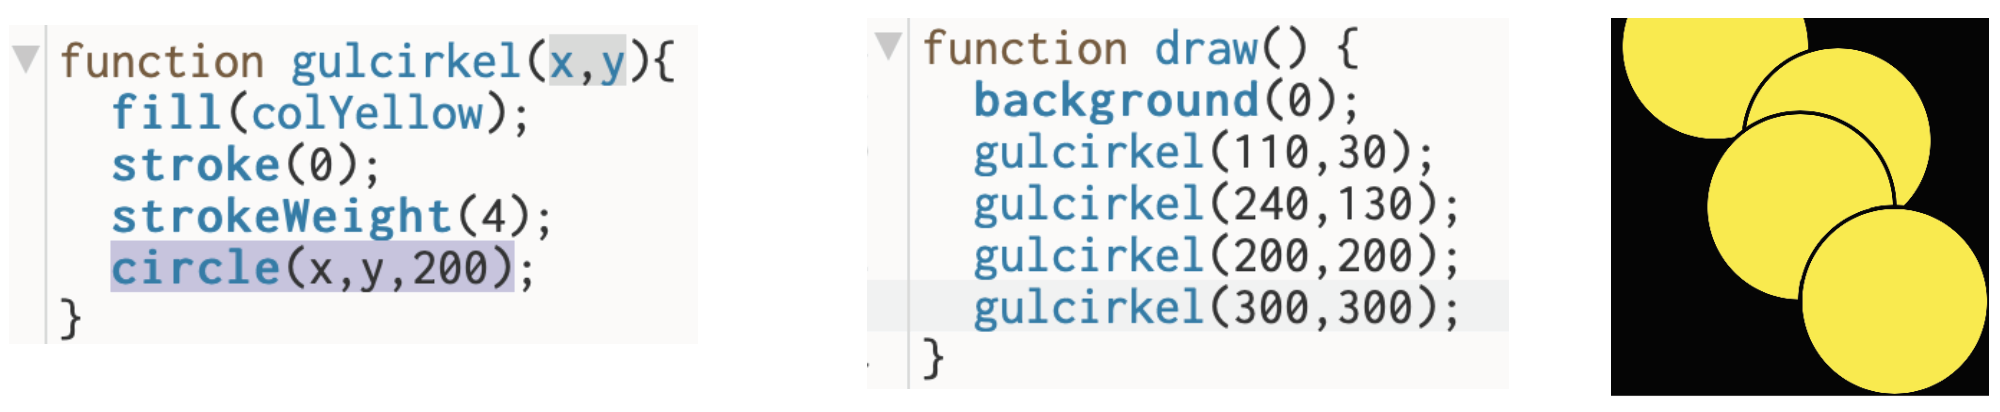
\includegraphics[width=0.7\textwidth]{billeder/treien.png} \\
Med overstående funktion kan jeg nemt tegne gule cirkle, lige hvor jeg \\

Du kan give din funktion ligeså mange input du har lyst til - og du må også gerne bruge navne i stedet for x, y, z. F.eks kunne man godt forestille sig at funktionen gulcirkel også tog et input der hed "diameter" og "farve": \textbf{gulcirkel(x, y, diameter, farve)}
\vspace{3mm}

\tcbsubtitle{Mikrofon}
Under setup tilføjes:\\


\includegraphics[width=0.4\textwidth]{billeder/micstart.png}\\

Nu lytter din computer med når du køre koden - hvis du altså husker at give den tilladelse. For f.eks. at få vist lydstyrken kan du nu i \textbf{draw()} skrive: \\

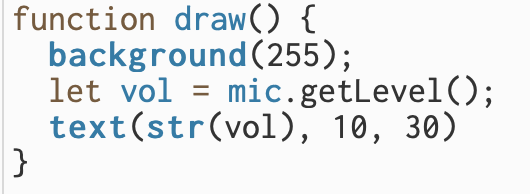
\includegraphics[width=0.35\textwidth]{billeder/vol.png}\\

\vspace{3mm}

\end{exercisebox}


\newpage

\begin{exercisebox}[adjusted title=En funktion der tegner med lyd]

Det er fristende at bruge mikrofonen til at genere noget på skærmen. Her er et simpelt eksempel på en funktion man kunne lave: \\

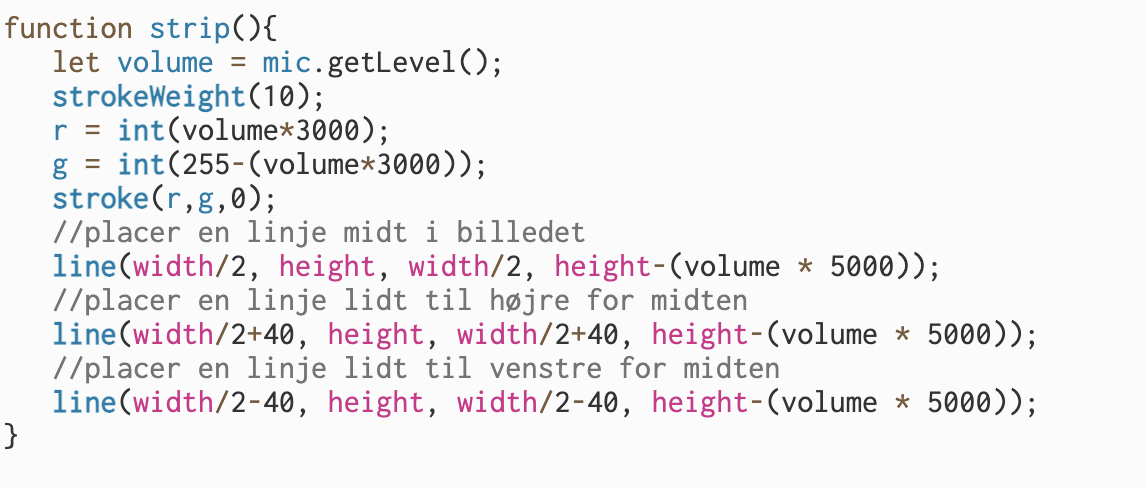
\includegraphics[width=0.9\textwidth]{billeder/tegnlyd.png}\\

For at se funktionen i brug, husk at kalde den under \textbf{draw()}.

\vspace{3mm}
\tcbsubtitle{En funktion der bruger en forløkke}
Man kan hurtigt få skabt masser af tegning ved at bruge en forløkke; et stykke kode der bliver kørt et bestemt antal gange. I følgende eksempel bruger jeg også funktionen \textbf{random()} for at ændre både størrelsen og farven på de ovaler jeg tegner. Derudover gør jeg cirklerne halvgennemsigtige ved at bruge \textbf{setAlpha(100)}: \\

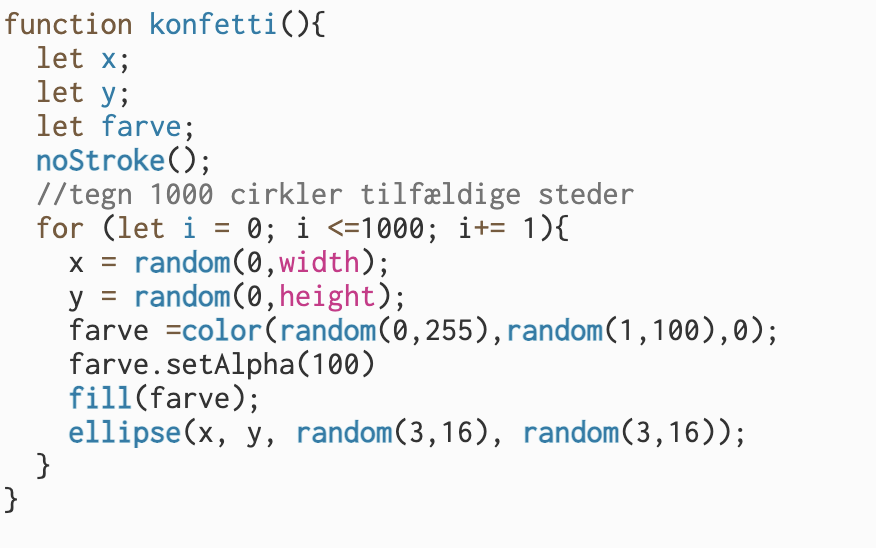
\includegraphics[width=0.8\textwidth]{billeder/tegnforloop.png}\\

For at se funktionen i brug, husk at kalde den under \textbf{draw()}.

\vspace{3mm}
\tcbsubtitle{Opgave}

\begin{itemize}
    \item Prøv at ændre på nogle af tallene og kør koden for at se hvad der sker. 
    \item Leg med udtryk og fyld dit videobillede godt op med tegninger og billeder. 
\end{itemize}

\vspace{3mm}
\end{exercisebox}


\begin{exercisebox}[adjusted title= Optimer koden på mac.]

I princippet kunne vi godt bare bruge det video-output vi har lavet i p5js, men det fungere lidt for langsomt til at give en god fornemmelse under et zoommøde, så vi vil hellere optage og bruge video fra OBS. For at gøre det skal vi have tilføjet computerens webcam. Tryk på + for at tilføje en ny \textbf{source}/\textbf{kilde} og vælg \textbf{Video Capture Device}/\textbf{videooptagelsesenhed}: \\

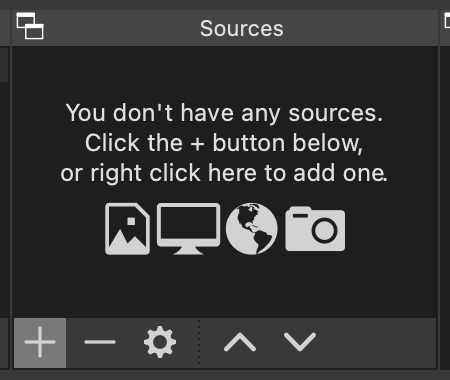
\includegraphics[width=0.2\textwidth]{billeder/OBSsourse.png}\\

Nu dukker en dialogboks op, hvor du klikker "OK". I den næste dialogboks der dukker op skal du under device vælge det kamera der er dit frontkamera og klikke ok. \\

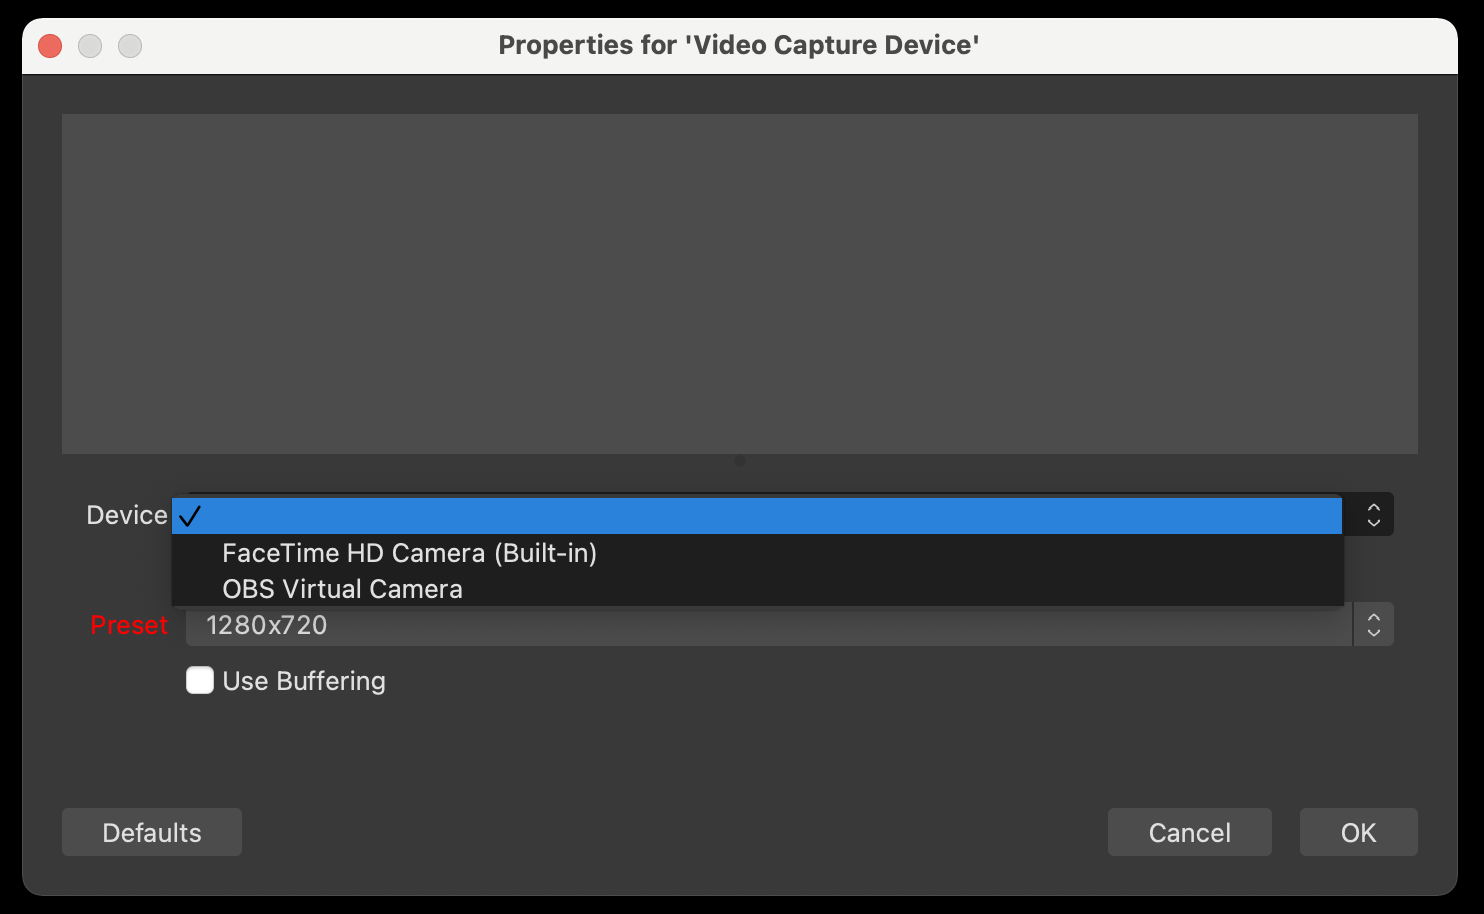
\includegraphics[width=0.7\textwidth]{billeder/velgdevise.png}\\

Nu skulle du gerne kunne se dig selv i OBS. \\
\tcbsubtitle{Særlig til Windowsbrugere}
\vspace{3mm}
Windows blokerer for at man kan bruge webkamera flere steder på een gang. Se appendix med titlen \textbf{Work-around til Windows} for en løsning. 
\vspace{3mm}
\end{exercisebox}

\newpage

\begin{exercisebox}[adjusted title= Klargør koden i p5.js - mac optimering]

Det var godt at få tegnet videoen sammen med billederne, så vi kunne placere billederne, men nu skal du ikke længere tegne din video under \textbf{draw()}. Du får programmet til at springe en linje over, ved at skrive "//" foran. 
Vi vil gerne have en "greenscreen" som baggrund til tegningerne - det gør det nemt at lægge dem ovenpå i OBS. Så; ændre baggrundsfarven til grøn.\\

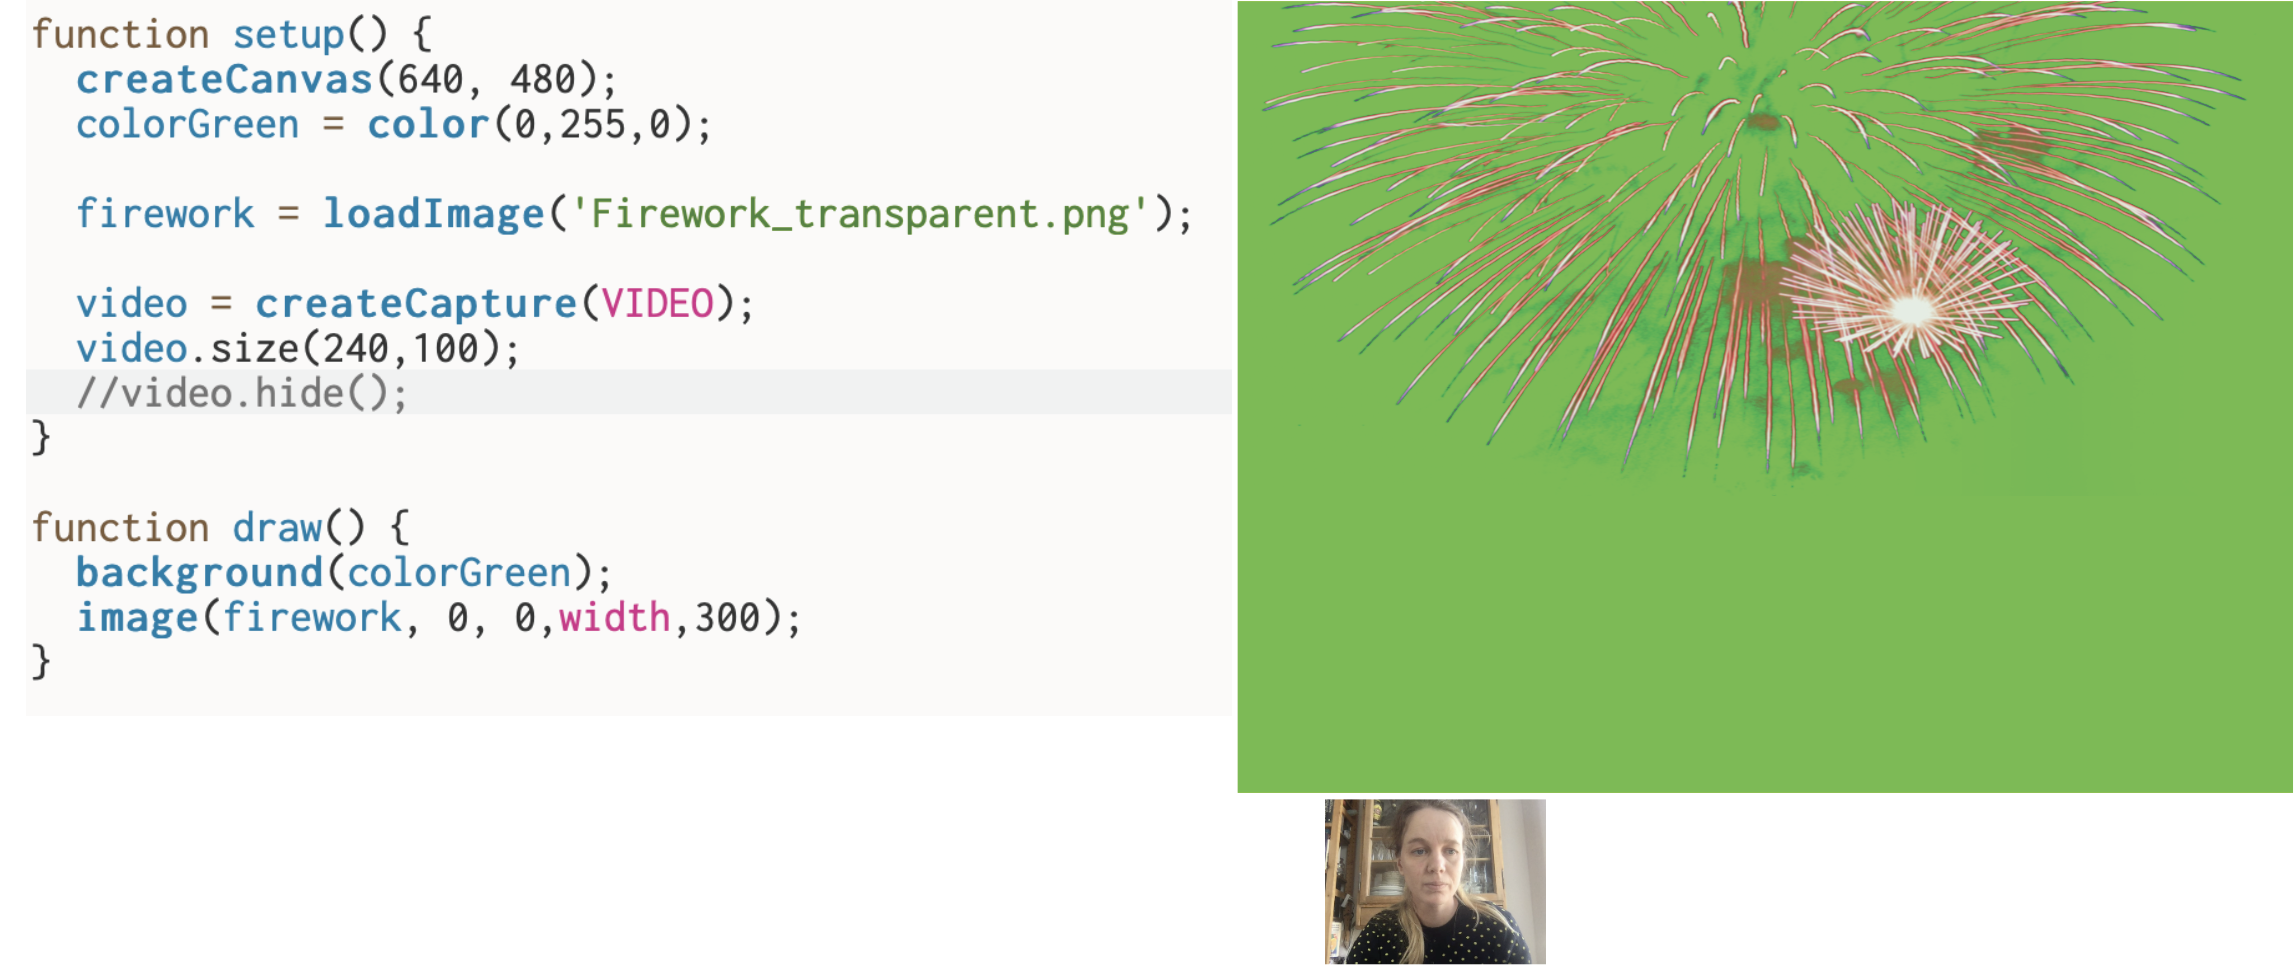
\includegraphics[width=0.8\textwidth]{nyebilleder/samleteksemple.png}\\

Hvis du gerne stadig vil kunne se dig selv, så kan du under \textbf{setup()} sætte størrelsen på video ned, og springe linjen med \textbf{video.hide()} over. \\


\tcbsubtitle{kombiner p5.js, OBS og Zoom}
\textbf{I p5.js:}\\
Du skal starte med at gemme din sketch. Under \textbf{file} vælges \textbf{save}. Vælg et passende navn. \\
Dernæst under \textbf{file} vælges \textbf{share} og \textbf{fullscreen}. Åben linket i et nyt vindue.  \\

%%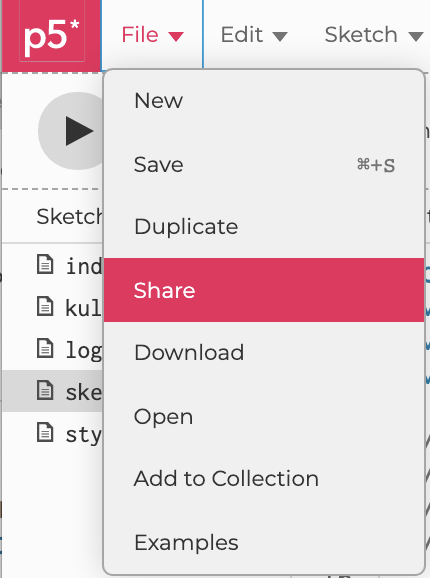
\includegraphics[width=0.1\textwidth]{billeder/share.png}\\

\textbf{I OBS:}\\
Nu skal du tilføje en ny \textbf{source}/\textbf{kilde} i OBS. Denne gang skal det være af typen \textbf{Window capture}/\textbf{vindue optagelse}. Vælg det vindue der kører din kode\\

Beskær billedet i OBS ved at holde "option" inde på mac eller "alt" på windows og træk i de røde punkter i rammen. Klip til så det kun er det grønne billede der ses. Du skalerer ved at trække i de røde punkter uden option. Få videobillede og p5.js billede til at passe så nogenlunde sammen.   \\

%%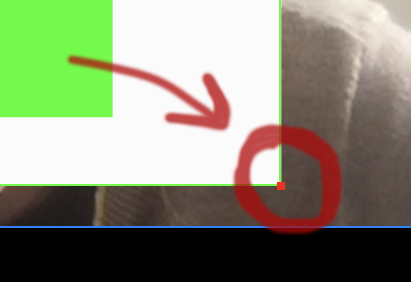
\includegraphics[width=0.1\textwidth]{billeder/roedpunkt.jpg}\\

Højre-klik på din "window capture"-source og vælg \textbf{filters}. Tilføj et nyt \textbf{effect filter} ved at klikke på plus og vælg \textbf{croma key}/\textbf{croma nøgle}. Default-instillingerne er til greenscreen, så du klikker bare ok.\\

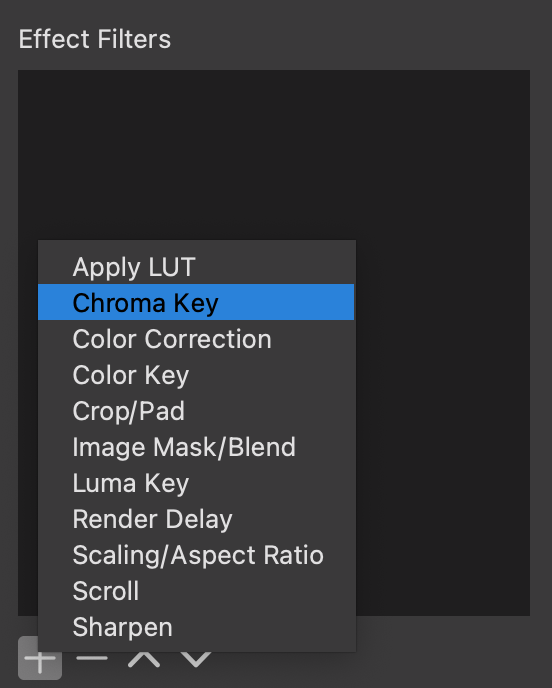
\includegraphics[width=0.1\textwidth]{billeder/cromakey.png}\\

Nu mangler du kun at starte virtuelt kamera i OBS (under \textbf{controls}/\textbf{styring}) \\

\textbf{I Zoom:}\\
Dit virtuelle kamera skulle gerne dukke op som et kamera der kan vælges i Zoom. Muligvis skal Zoom genstartes.

\end{exercisebox}


\begin{exercisebox}[adjusted title= Work-around til Windows]
En feature ved Windows, er at man kun kan bruge web-kamera i een app eller browser ad gangen. Det er lidt en udfordring, da vi gerne skulle bruge det uafhængigt af hinanden i hhv p5.js og OBS.\\

Det første du skal være opmærksom på at at du ikke kan have teachablemachine kørende i baggrunden samtidig med at du bruger OBS. Det næste er problemet med at bruge kamera i p5.js samtidig med OBS.\\

Løsningen her og nu bliver at starte det virtuelle kamera i OBS, og så bruge det som input i p5.js.\\

Når du har sketchen åben i Crome og trykker  
\includegraphics[height=5mm]{ikoner/run.png} dukker et lille videokamera-ikon op til højre i adressefeltet. 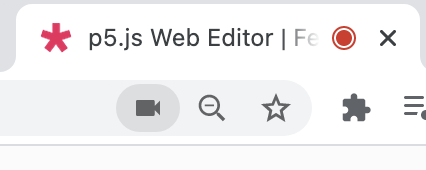
\includegraphics[height=10mm]{nyebilleder/videoikon.png} tryk på det og vælg \includegraphics[height=10mm]{nyebilleder/managevidoe.png}. \\

Nu skulle du gerne komme til det sted i settings hvor du kan vælge mellem dit indbyggede kamera og det virtuelle. \includegraphics[height=20mm]{nyebilleder/virtuel.png} Ulempen her er at når der popper et billede op, som følge af dine bevægelser, så genkender den ikke længere bevægelse og billedet bliver taget ned igen. Det giver stadig en sjov effekt, men også lidt benspænd til de kunstneriske udfoldelser.  
\vspace{3mm}

\end{exercisebox}


\newpage
\begin{exercisebox}

\includegraphics[width=0.6\textwidth]{nyebilleder/setupmodel.png}\\

\tcbsubtitle{Brug af biblioteker}
Åbn menuen med dine sketchfiles.\\

I sketchfiles ligger en fil der hedder \textbf{index.html}. Den skal du klikke på. Nu sletter du alt hvad der står, og skriver følgende: (du må gerne copy-paste)

\begin{Verbatim}[fontsize=\tiny]

<html>

<head>
  <meta charset="UTF-8">
  <script src="https://cdnjs.cloudflare.com/ajax/libs/p5.js/0.9.0/p5.min.js"></script>
  <script src="https://cdnjs.cloudflare.com/ajax/libs/p5.js/0.9.0/addons/p5.dom.min.js"></script>
  <script src="https://unpkg.com/ml5@latest/dist/ml5.min.js" type="text/javascript"></script>
  <script src="https://cdnjs.cloudflare.com/ajax/libs/p5.js/1.2.0/addons/p5.sound.min.js"></script>
</head>

<body>
  <script src="sketch.js"></script>
  <style>
    body {
      background: #FFF;
    }
  </style>
</body>
    
\end{Verbatim}

Nu vender du tilbage til din kode ved at klikke på \textbf{sketch.js} \\ Det vi har gjort her er, at vi har gjort nogle biblioteker tilgængelige, der ikke ligger som standard i p5.js. Vi skal bruge biblioteket til at klassificere vores video. \\
Tilføj linjerne med 'label' og 'classifier' til \textbf{setup()}:\\

\includegraphics[width=0.8\textwidth]{nyebilleder/withclassifier.png} \\

\textbf{classifier} er nu bundet op på din specifikke model. \textbf{label} er den variabel hvor vi gemmer det som vores videobillede bliver genkendt til. 

\end{exercisebox}

\newpage


\begin{exercisebox}[adjusted title= Vi er der næsten nu]

For at få det hele til at virke skal du bruge disse to funktioner. Det er dem der bruges til at identificere billederne fra videokamerareet og gemme resultatet i 'label'. Du skriver dem ind, helt i bunden af din sketch, præcis som de står her
\vspace{3mm}
\tcbsubtitle{classifyVideo()}
\vspace{3mm}

\includegraphics[width=0.8\textwidth]{billeder/classifyvideo.png} \\

\vspace{3mm}
\tcbsubtitle{gotResult(error, results)}

\includegraphics[width=0.6\textwidth]{billeder/gotresult.png} \\

\vspace{3mm}

\tcbsubtitle{Start classifier}

Nu mangler classifieren bare at blive startet under \textbf{setup()}. Skriv \textbf{classifyVideo()} nederst i setup, før den afsluttende \textbf{\}}.
\\

\textbf{setup()} skulle gerne se cirka sådan her ud nu, på nuværende tidpunkt: \\

\includegraphics[width=0.9\textwidth]{nyebilleder/helesetup.png} \\

\end{exercisebox}
\end{document}